% Created 2011-10-20 Thu 14:48
\documentclass{book}


\usepackage{leonine,amsmath,amssymb,amsthm,graphicx,setspace, hyperref, color}
\renewcommand{\thechapter}{\Roman{chapter}}
\newcommand{\bow}[1]{\colorbox{black}{\color{white} #1}}
\newcommand{\experiment}[1]{\bow{This section's results can be recreated by running #1}}
\providecommand{\alert}[1]{\textbf{#1}}
\begin{document}



\title{Experimental Results and Notes}
\author{Eric Purdy}
\date{20 October 2011}
\maketitle

\setcounter{tocdepth}{3}
\tableofcontents
\vspace*{1cm}


\chapter{What do I have to do?}
\label{sec-1}


\begin{itemize}
\item define etc. models
\item find objects in images

\begin{itemize}
\item why is this so hard???
\end{itemize}

\item do something with time series
\item learn parameters
\item show some sort of performance gain in classification?
\item learn structure
\end{itemize}
\chapter{Plan}
\label{sec-2}

\setcounter{section}{-1}
\section{Assembling Datasets}
\label{sec-2_1}
\subsection{Articulator}
\label{sec-2_1_1}
\subsection{Romer}
\label{sec-2_1_2}
\subsection{Weizmann horse dataset}
\label{sec-2_1_3}
\subsection{Hand datasets/ASL alphabet}
\label{sec-2_1_4}
\subsection{LabelMe}
\label{sec-2_1_5}
\subsection{Time series datasets}
\label{sec-2_1_6}
\section{Grammatical Shape Models}
\label{sec-2_2}
\subsection{Compare shape grammars to other point-set models}
\label{sec-2_2_1}

We are building probabilistic models of shape. We want to demonstrate
that our models have nice properties. In particular, we would like to
prove that our models do as well or better in explaining geometric
variability, compared to other popular models of shape. For now, we
consider only models of shape that deal with the location in the plane
of a fixed number of corresponding landmarks, $z_1, \dots, z_n$.

The easiest way to compare two generative probabilistic models is to
examine samples from them, and subjectively assess their similarity to
real data. This is inherently a very qualitative evaluation.

When the other models are also probabilistic models, we can compare
them in a more quantitative way using (estimated) cross-entropy, which
is defined as
$$H(\{x_1,\dots,x_n\}, q) = - \sum_{i=1}^n \frac{1}{N} \log_2 q(x_i).$$

If $X = \{x_1,\dots,x_n\}$ is unseen data, and a large enough sample
to be statistically useful, then $H(X,q)$ is a good measure of how
well a model explains unseen data. Smaller values of $H(X,q)$ suggest
that $q$ is a better model. One problematic aspect of cross-entropy is
that it is only meaningful if $q$ is a correctly normalized
probability distribution. Often it is easier to compute
$\widetilde{q}(x) = Z\cdot q(x)$ for some unknown but fixed constant
$Z$.

When we are comparing to a non-probabilistic model, sampling is
impossible, and cross-entropy is meaningless. In this case, the most
straightforward way to compare models is by using them both in some
task like classification. For instance, we can use both models to
classify leaves as being either oak or maple leaves. Whichever model
has a lower error rate is better capturing the differences between the
two classes of shapes.

We would like to consider the following models:

\begin{itemize}
\item Markov curve models, where we represent a curve as a series of
    turns and line segments (a la the Logo turtle), and then add noise
    to the angle of each turn, and the length of each line segment.
\item Procrustes-type models, such as the Watson distribution and the
    Bingham distribution
\item Independent gaussian perturbations of each point
\item Independent nonparametric perturbations of each point
\end{itemize}

For our models, we would like to consider several different models:
\begin{itemize}
\item a hand-built model
\item a model automatically inferred from a single example
\item a model automatically inferred from a single example and tuned
    with multiple examples
\end{itemize}
\subsection{Model curves of varying length}
\label{sec-2_2_2}

We would like to demonstrate that shape grammars effectively model
curves with varying numbers of points. This is important to achieve
scale invariance, since larger objects will generally have more
detailed boundaries.

For this question, there are fewer standard probabilistic models to
compare grammars to. There are many discriminative models that deal
with curves of varying length. Unfortunately, there are few
classification tasks hard enough to distinguish between different
models. There are more classification tasks when we consider the more
restricted problem of comparing two different shapes, rather than
modeling an entire class and classifying a single shape.

We can examine samples from variable-length grammar models, and we can
try to perform well on classification tasks.

One hard matching task is MPEG-7. We are only allowed to compare
images in pairs, and there are about 2 million pairs that must be
iterated over. Therefore, we must be able to build a grammar from a
single example that is very small and very robust. We must also be
able to make coarse versions of curves that are good stand-ins, since
we will have to lessen the work required to parse. We can start with a
much smaller subset of the dataset, of course.
\subsection{Build more interesting grammars}
\label{sec-2_2_3}

We would like to demonstrate the expressiveness of grammatical curve
models. In particular, we would like to show that a hand-built grammar
can exhibit interesting variation, such as:
\begin{itemize}
\item articulating parts of an object
\item the presence or absence of a part
\item a choice between two different variations on the part
\item shared parts that occur in different contexts
\end{itemize}

We will show samples from these models.

We also want to do this with automatically inferred grammars, but that
is a hard problem. Section 6 will document our efforts there.
\section{Parsing}
\label{sec-2_3}

Given a grammar model and a curve, we want to calculate how likely the
curve is under the model, and we would like to extract the most likely
correspondence between the points of the curve and the parts of the
model. We demonstrate parsing with several different tasks:
\begin{itemize}
\item Given two curves whose points can be put into a one-to-one
    correspondence, show that we can recover that correspondence by
    building a grammar model from one curve and using it to parse the
    other. We can do this either with a hand-built model or an
    automatically generated model.
\item Given a coarse curve and a finer curve, show that we can recover a
    reasonable correspondence between the points of the coarse curve
    and a subset of the points of the finer curve. We do this by
    building a grammar model from the coarse curve and using it to
    parse the finer curve. This demonstrates that we can model longer
    curves than were used to build the grammar.
\item Given a coarse curve and a finer curve, recover a reasonable
    correspondence by building a grammar from the finer curve and
    parsing the coarse curve. This demonstrates that we can model
    shorter curves than were used to build the grammar.
\item Given a coarse curve and a finer curve, where the finer curve has
    features not present in the coarse curve (such as bumps or pits),
    recover a reasonable correspondence by building a grammar from the
    coarse curve and using it to parse the finer curve. This
    demonstrates that we can model longer curves that have non-trivial
    variation in detail.
\item Given two fine curves which do not have a perfect correspondence,
    recover a reasonable correspondence by building a grammar from one
    and using it to parse the other. This demonstrates that we can
    model both extra and missing points.
\item Given a rich grammar, show that we can choose the correct
    structure for input curves.
\end{itemize}
\section{EM}
\label{sec-2_4}

Given a fixed grammar structure (the symbols and rules), we can
optimize the parameters (rule probabilities and midpoint
distributions). EM is an iterative algorithm for improving the
parameters of a probabilistic model when important information (in our
case, the ``true'' parses) is unobserved.

We wish to demonstrate that EM works to tune the parameters of a shape
grammar. We would like to do the following:
\begin{itemize}
\item Tune a simple hand-built grammar using several curves of fixed
    length, and then show that it produces reasonable samples, and
    that the cross-entropy estimated on unseen data is improved by EM.
\item Tune a simple hand-built grammar using several curves of fixed
    length. Start with a grammar that has several choices of midpoint
    for each of its rules, to allow for greater geometric
    variation. Show that it produces reasonable samples, and that the
    cross-entropy estimated on unseen data is improved by EM.

    We would also like to do this for a slightly more complicated
    grammar, in which the choice of midpoint at a high level can
    influence the choice of midpoint at lower levels.
\item Tune a hand-built grammar that exhibits structural variation.
\item We would like to show that EM does badly when it starts with bad
    parses.
\end{itemize}
\section{Parsing in Cluttered Images}
\label{sec-2_5}

Given a shape model and an image containing a similar shape, we would
like to be able to find the shape in the image. This is done by
searching for a shape that is rated highly by the shape model, and for
which evidence exists in the image.

We will work on solving harder and harder versions of this problem:
\begin{itemize}
\item Take a known curve, and generate evidence that suggests that
    curve, and no other curve. Find the curve.
\item As above, but randomly add evidence to other parts of the image.
\item Extract evidence from an actual image, and use this to find the
    curve.
\end{itemize}
\section{Using SDF's in Other Domains}
\label{sec-2_6}

This question is pretty orthogonal to everything else.
\section{Learning Structure}
\label{sec-2_7}
\subsection{Figure out optimal single-example grammar}
\label{sec-2_7_1}
\subsection{Implement Merge and Replace}
\label{sec-2_7_2}
\subsection{Implement Merge and Replace KL heuristics}
\label{sec-2_7_3}
\subsection{Use Merge and Replace to search for good grammar}
\label{sec-2_7_4}
\subsection{Figure out how to optimally incorporate new samples}
\label{sec-2_7_5}
\section{Learning Texture}
\label{sec-2_8}
\subsection{Learn a texture-only grammar}
\label{sec-2_8_1}
\subsection{Learn a grammar that combines global shape with local texture}
\label{sec-2_8_2}
\chapter{Results}
\label{sec-3}

\setcounter{section}{-1}
\section{Assembling Datasets}
\label{sec-3_1}
\subsection{Synthetic Datasets}
\label{sec-3_1_1}

\begin{itemize}
\item Polygons:
\end{itemize}

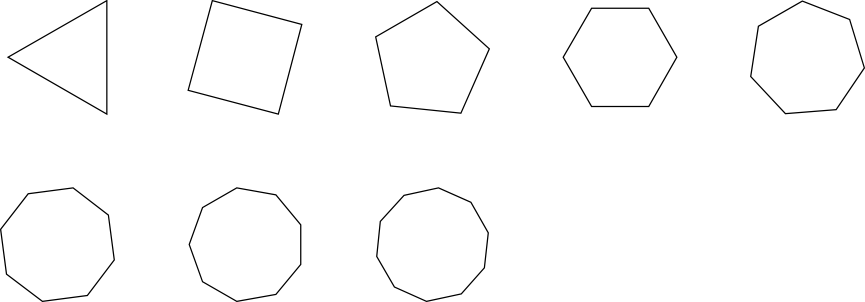
\includegraphics[width=4in]{./0.datasets/synth/output.d/polygons.eps}

\begin{itemize}
\item Stars:
\end{itemize}

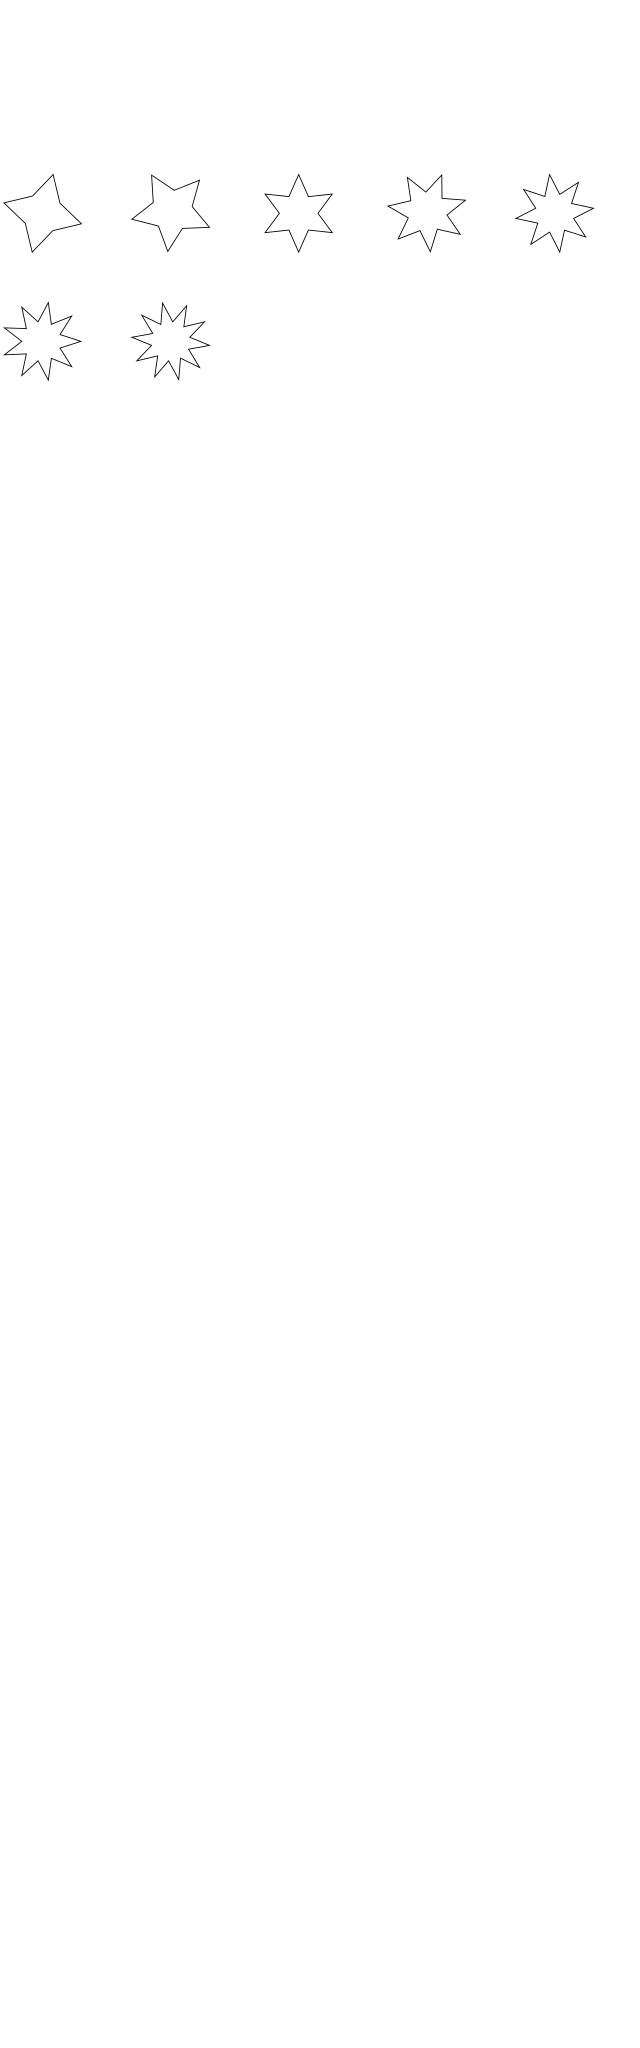
\includegraphics[width=4in]{./0.datasets/synth/output.d/stars.eps}

\begin{itemize}
\item A shape with an articulating arm:
\end{itemize}

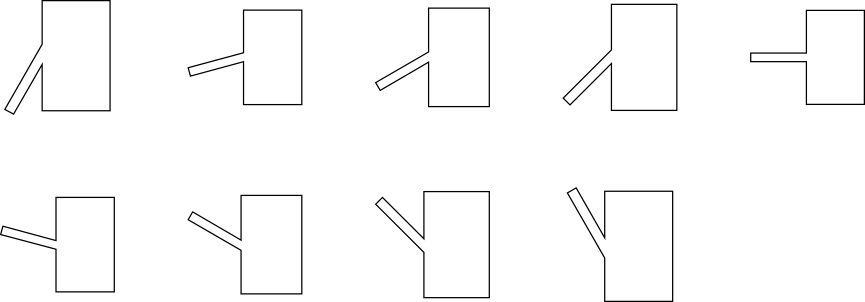
\includegraphics[width=4in]{./0.datasets/synth/output.d/articulator.eps}

\begin{itemize}
\item These are 6-armed shapes, where each arm can have one of two
    shapes.
\end{itemize}

\includegraphics[width=4in]{./0.datasets/synth/output.d/narms.eps}
\subsection{Romer}
\label{sec-3_1_2}

\begin{itemize}
\item We have hand-annotated a simplified version of Romer by
    hand-marking 27 points on a number of images
\end{itemize}
%\% \#+CAPTION:    Hand-annotated simplified Romer dataset
%\% \#+ATTR_\LaTeX{}: width=6in placement=[h!]
\includegraphics[width=4in]{./0.datasets/romer/output.d/romerI.eps}

\begin{itemize}
\item Also have the ``ground-truth'' curves that come from diffing images
    with the background, although they are actually quite messy
\end{itemize}
%\% \#+CAPTION:    ``Ground truth'' curves from Romer dataset
\includegraphics[width=4in]{./0.datasets/romer/output.d/romerII.eps}
\begin{itemize}
\item The images themselves
\end{itemize}
\subsection{Swedish Leaves}
\label{sec-3_1_3}


\begin{itemize}
\item 
\end{itemize}
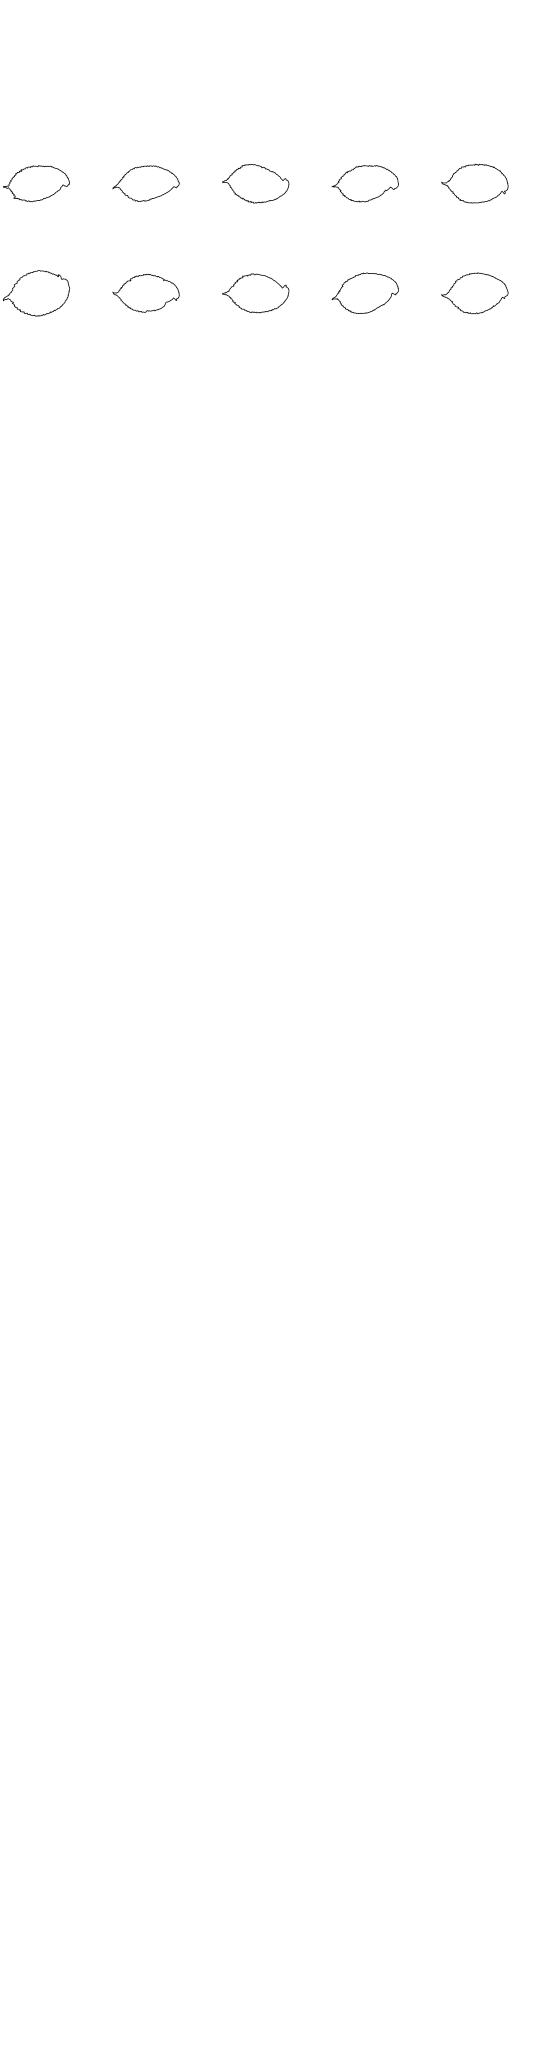
\includegraphics[width=4in]{./0.datasets/leaves/output.d/leaves_01.eps}

\begin{itemize}
\item 
\end{itemize}
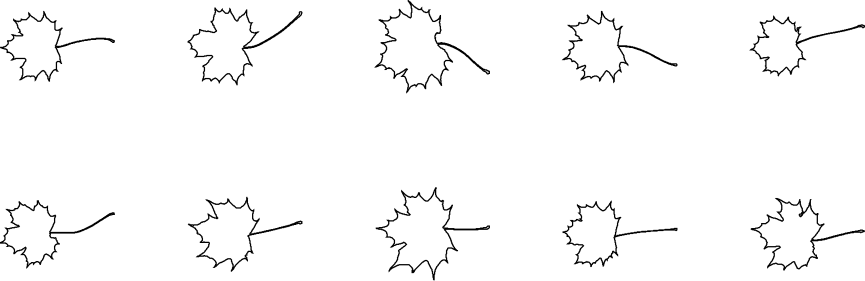
\includegraphics[width=4in]{./0.datasets/leaves/output.d/leaves_02.eps}

\begin{itemize}
\item 
\end{itemize}
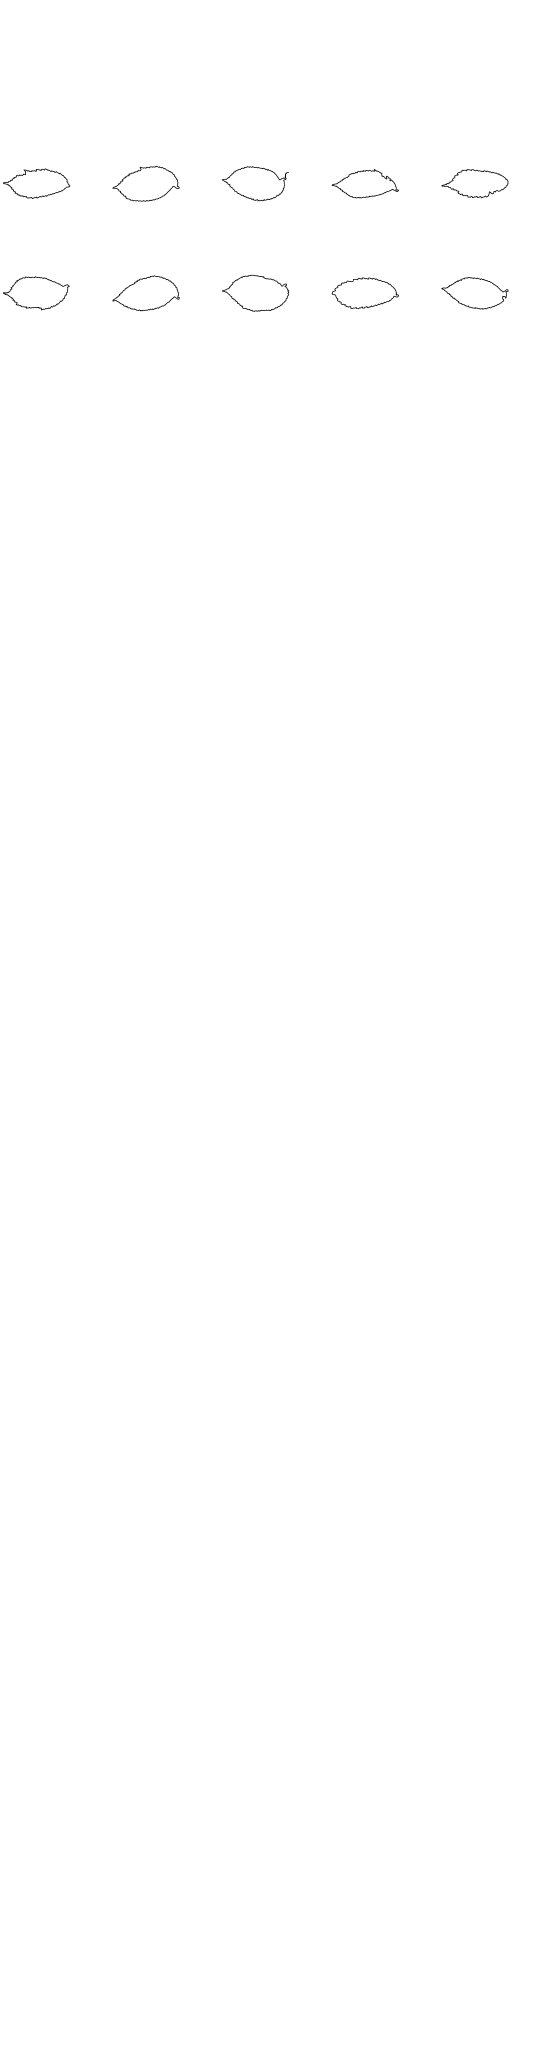
\includegraphics[width=4in]{./0.datasets/leaves/output.d/leaves_03.eps}

\begin{itemize}
\item 
\end{itemize}
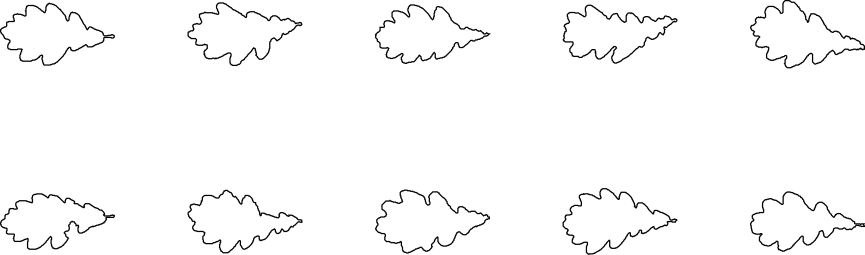
\includegraphics[width=4in]{./0.datasets/leaves/output.d/leaves_04.eps}

\begin{itemize}
\item 
\end{itemize}
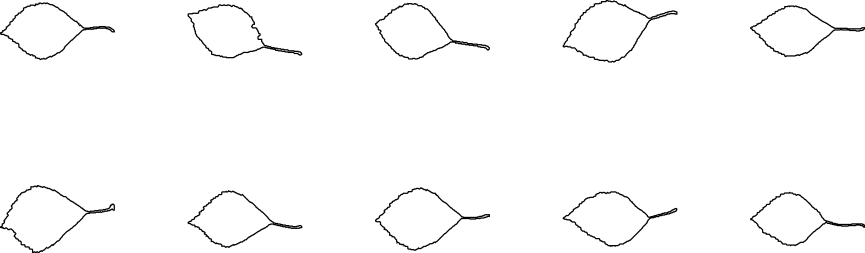
\includegraphics[width=4in]{./0.datasets/leaves/output.d/leaves_05.eps}

\begin{itemize}
\item 
\end{itemize}
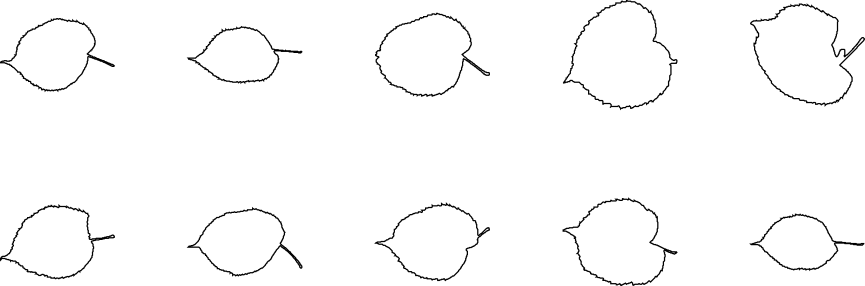
\includegraphics[width=4in]{./0.datasets/leaves/output.d/leaves_06.eps}

\begin{itemize}
\item 
\end{itemize}
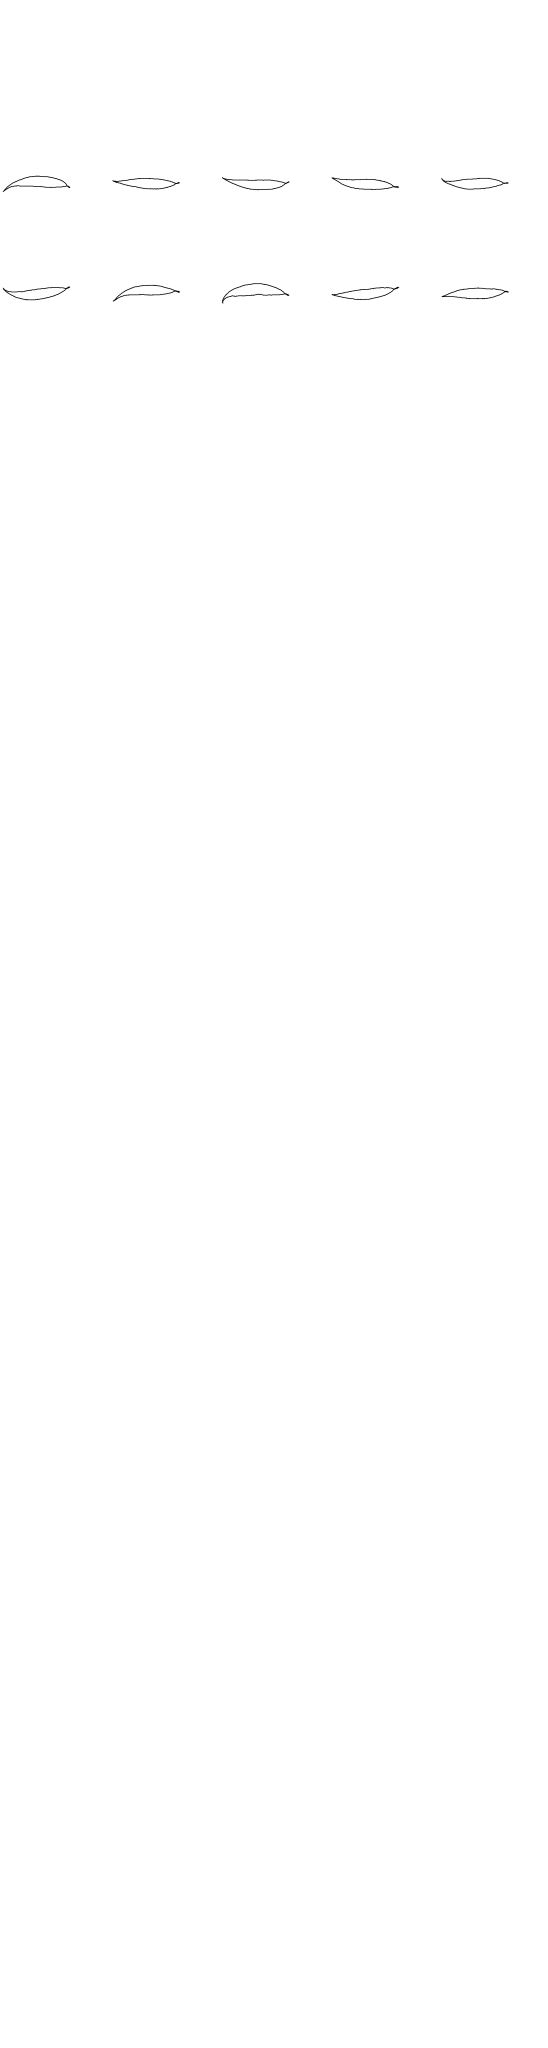
\includegraphics[width=4in]{./0.datasets/leaves/output.d/leaves_07.eps}

\begin{itemize}
\item 
\end{itemize}
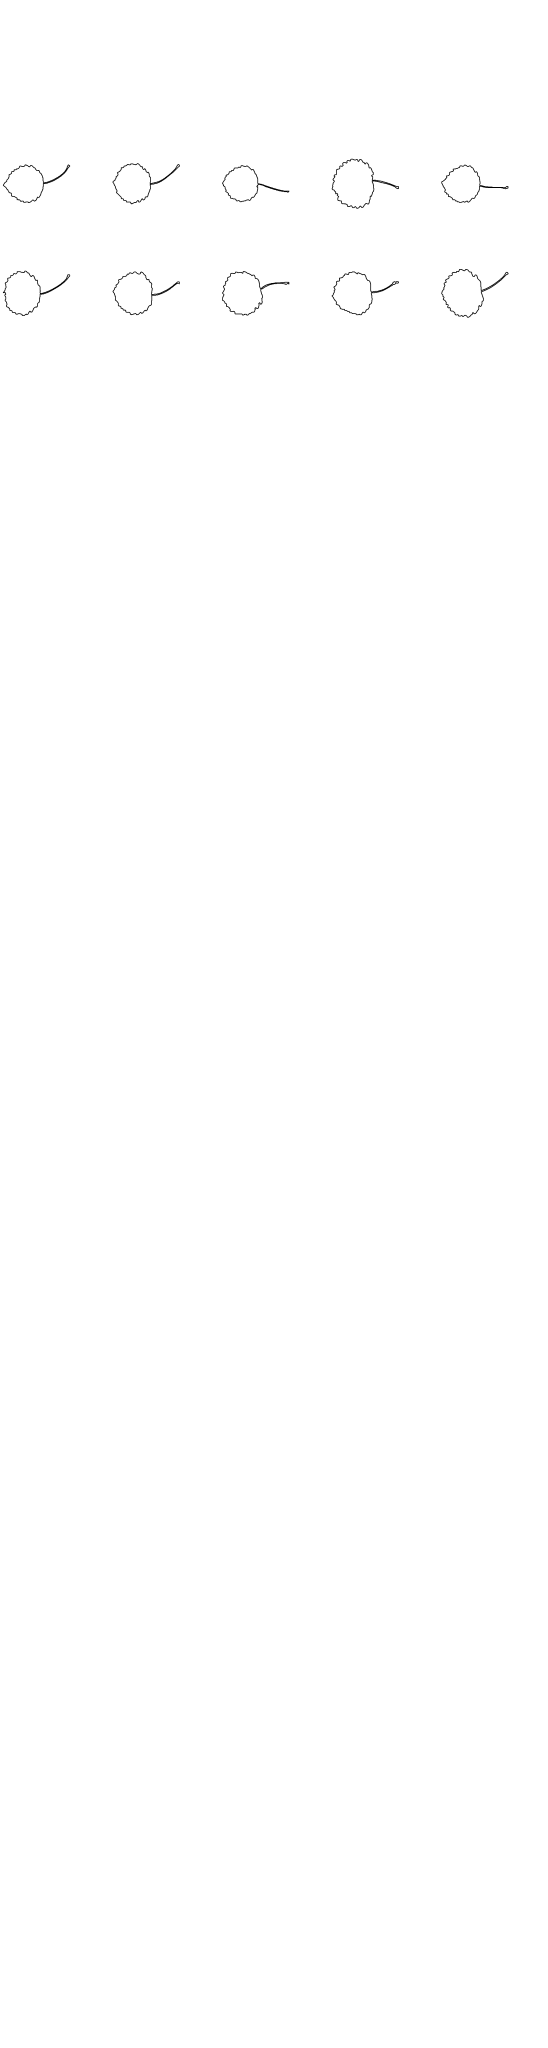
\includegraphics[width=4in]{./0.datasets/leaves/output.d/leaves_08.eps}

\begin{itemize}
\item 
\end{itemize}
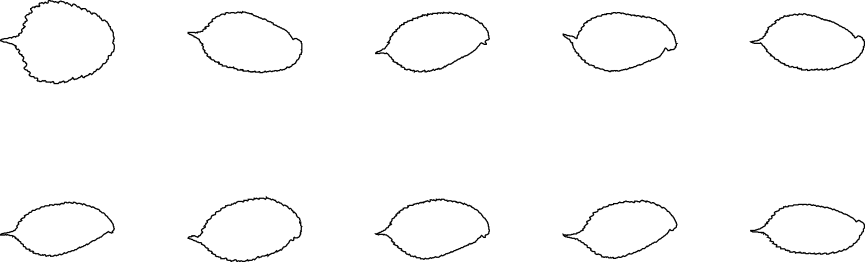
\includegraphics[width=4in]{./0.datasets/leaves/output.d/leaves_09.eps}

\begin{itemize}
\item 
\end{itemize}
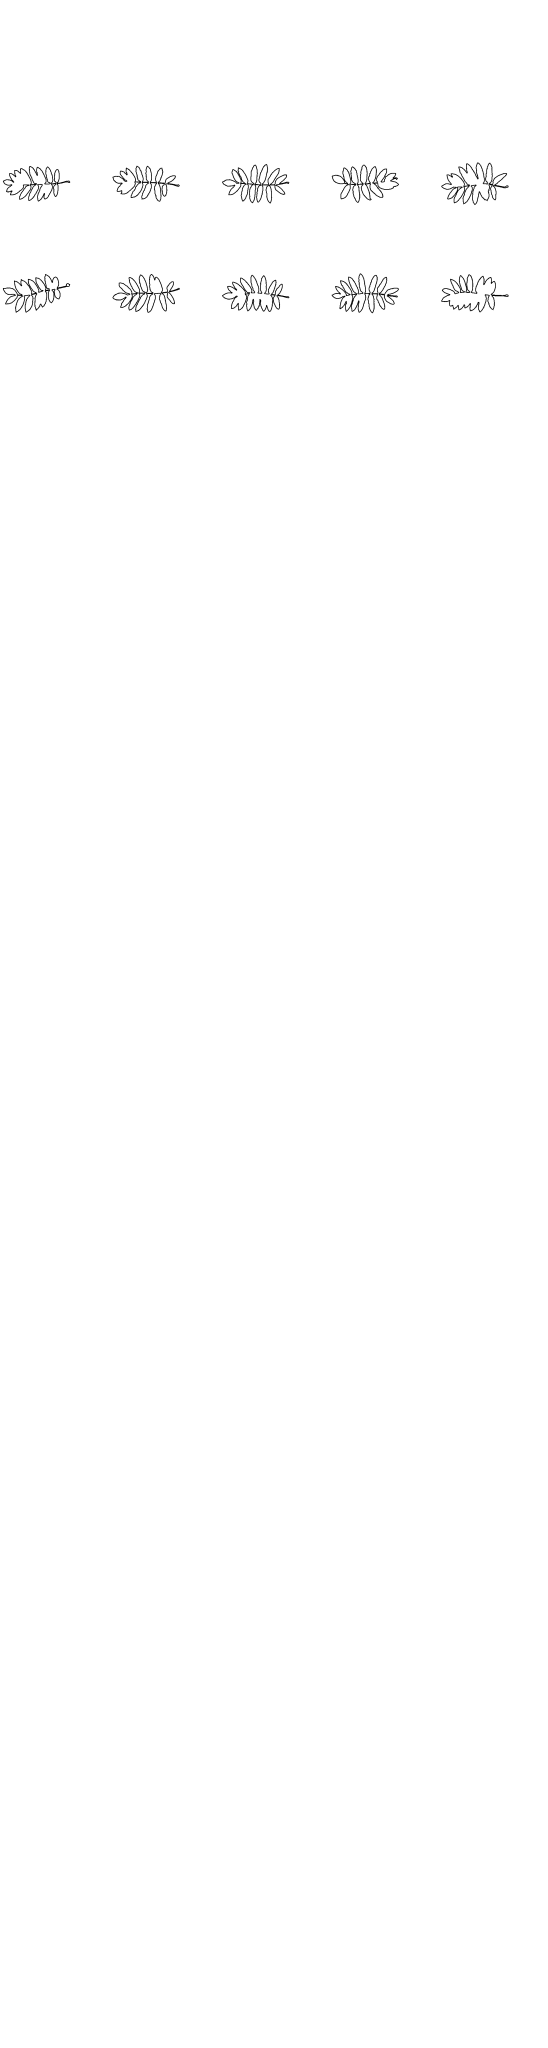
\includegraphics[width=4in]{./0.datasets/leaves/output.d/leaves_10.eps}

\begin{itemize}
\item 
\end{itemize}
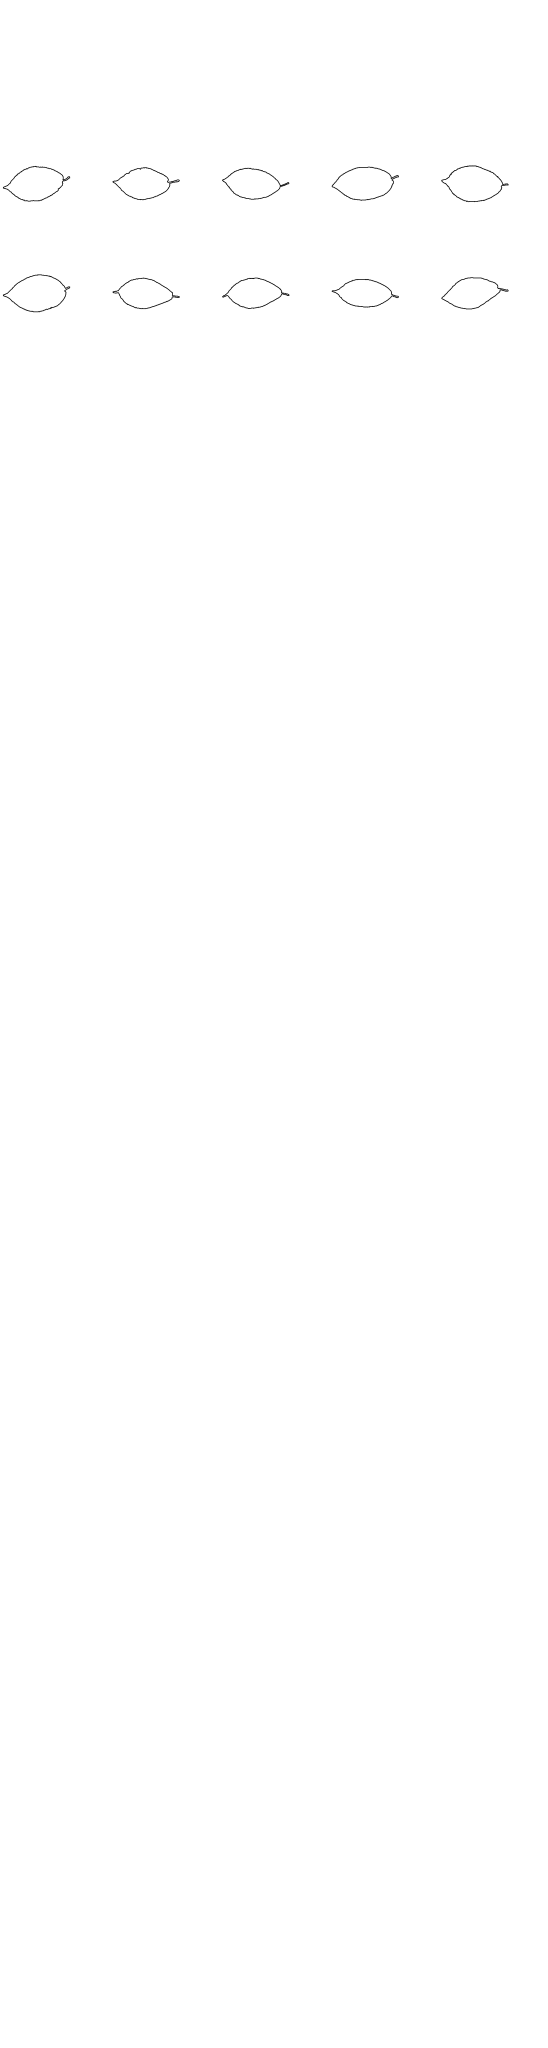
\includegraphics[width=4in]{./0.datasets/leaves/output.d/leaves_11.eps}

\begin{itemize}
\item 
\end{itemize}
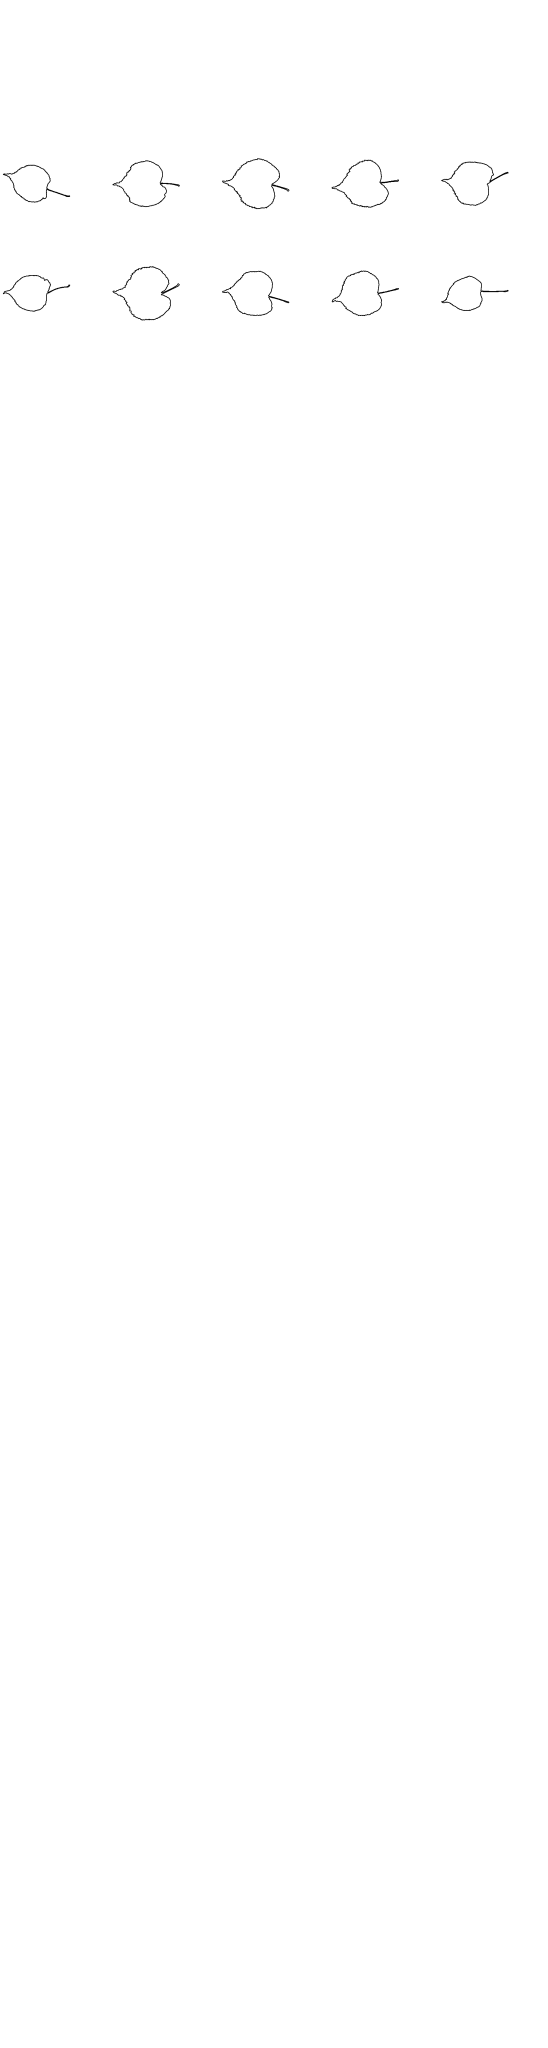
\includegraphics[width=4in]{./0.datasets/leaves/output.d/leaves_12.eps}

\begin{itemize}
\item 
\end{itemize}
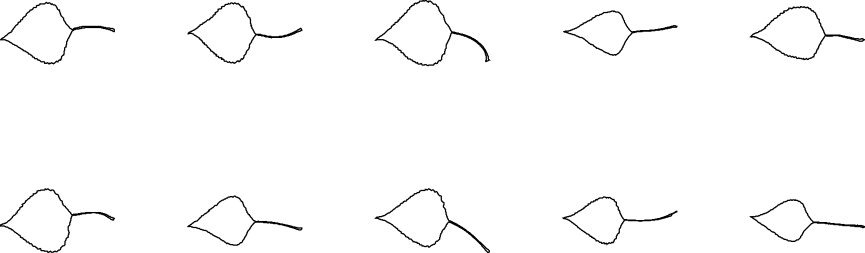
\includegraphics[width=4in]{./0.datasets/leaves/output.d/leaves_13.eps}

\begin{itemize}
\item 
\end{itemize}
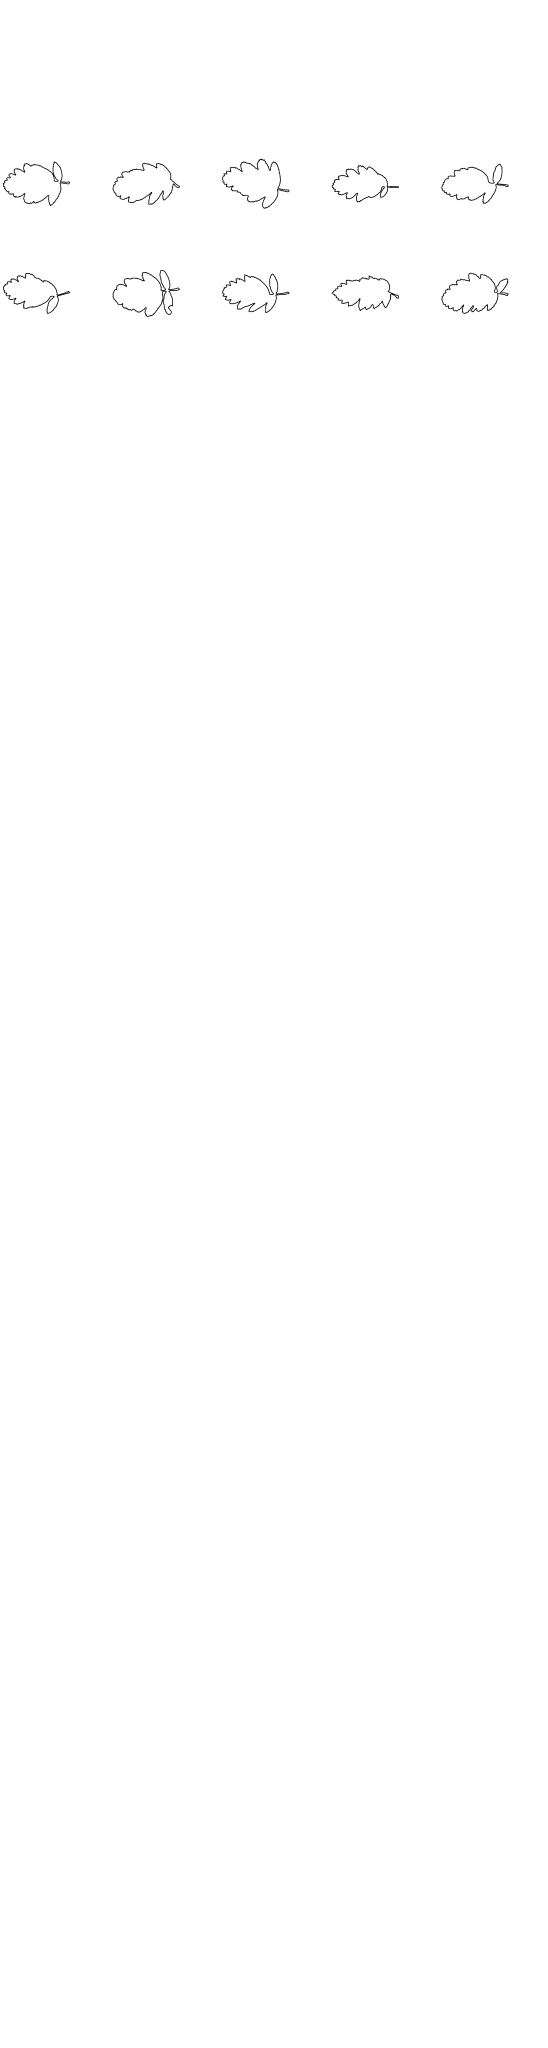
\includegraphics[width=4in]{./0.datasets/leaves/output.d/leaves_14.eps}

\begin{itemize}
\item 
\end{itemize}
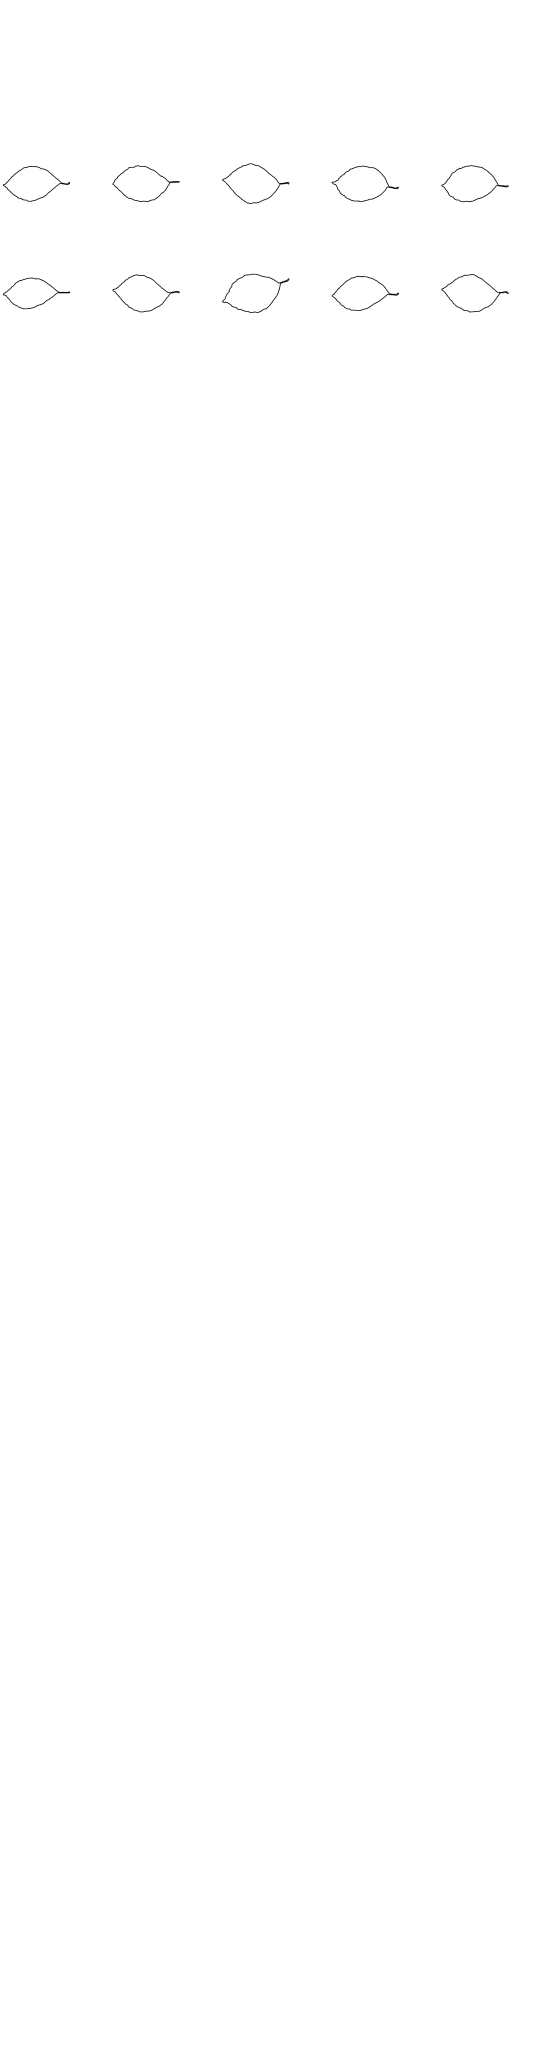
\includegraphics[width=4in]{./0.datasets/leaves/output.d/leaves_15.eps}
\section{Grammatical Shape Models}
\label{sec-3_2}
\subsection{Make sure Watson distribution is reasonable}
\label{sec-3_2_1}

\experiment{1.grammars/test\_watson/test\_watson.py}

In the following experiments, we select a random triangle (by using a
Gaussian in Bookstein coordinates). We then draw 20 samples from the
Watson distribution centered at this triangle (using 30 for the
concentration parameter of the Watson). We then reestimate the Watson
distribution from the samples.

This is a less noisy version of the learning task that EM faces when
refitting the midpoint distributions of a grammar from 20 samples.

\begin{table}
\begin{tabular}{l l l}
number of samples & mean & concentration\\ 
\hline
(true) & 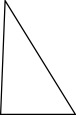
\includegraphics[width=0.6in]{output/1.models/samples_watson/watson_true.png} & 30.00\\ 
\hline
3 & 
\includegraphics[width=0.6in]{output/1.models/samples_watson/watson_est_3.png} & 19.37 \\ 
10 & 
\includegraphics[width=0.6in]{output/1.models/samples_watson/watson_est_10.png} & 37.72 \\ 
30 & 
\includegraphics[width=0.6in]{output/1.models/samples_watson/watson_est_30.png} & 32.75 \\ 
100 & 
\includegraphics[width=0.6in]{output/1.models/samples_watson/watson_est_100.png} & 27.66 \\ 
300 & 
\includegraphics[width=0.6in]{output/1.models/samples_watson/watson_est_300.png} & 28.11 \\ 
1000 & 
\includegraphics[width=0.6in]{output/1.models/samples_watson/watson_est_1000.png} & 26.62 \\ 
\end{tabular}
\caption{Fitting the Watson distribution with different numbers of samples.}
\end{table}

\subsection{Build an interesting grammar by hand}
\label{sec-3_2_2}

\experiment{1.grammars/handbuilt/handbuilt.py}

Here we are drawing a grammar. We have built this grammar by hand, by
taking the following curve, and specifying a decomposition of it:

%\% \#+CAPTION:    The initial curve
\includegraphics[height=2in]{./1.grammars/hand_built/output.d/hand_built_curve.eps}

Here is the decomposition:

\includegraphics[width=5in]{./1.grammars/hand_built/output.d/hand_built_sdf.eps}

Here is the grammar:

Here are some samples from the grammar:

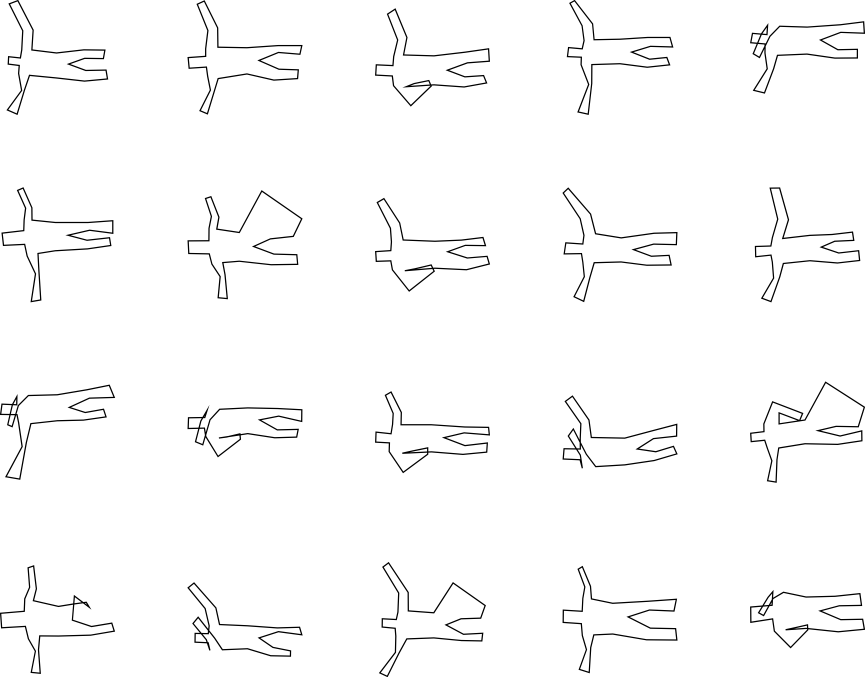
\includegraphics[width=6in]{output/3.learning/incremental/gram.19.d/samples.png}


\section{Parsing}
\label{sec-3_3}
\subsection{One-to-one}
\label{sec-3_3_1}


Here we have two curves given by hand-annotation of the Romer
dataset. We build a grammar from the curve on the left, using a
hand-built set of constituents. We then parse the curve on the right,
and show the Viterbi parse by showing the correspondences between the
two curves.

Because there are no missing or extra points, this is straightforward.

%\% \#+CAPTION:    On the left, the model curve. On the right, the parsed curve
\includegraphics[width=6in]{./2.parsing/one_to_one/output.d/parse.eps}
\subsection{Recover a correspondence with extra intermediate points}
\label{sec-3_3_2}


We build a grammar from a single example from the hand-annotated Romer
dataset, and use it to parse a curve from the ground-truth Romer
dataset. We successfully recover a very reasonable correspondence.

%\% \#+CAPTION:    On the left, the model curve. On the right, the parsed curve
\includegraphics[width=6in]{./2.parsing/longer_curves/output.d/parse.eps}


\begin{itemize}
\item The ground-truth Romer curve has more intermediate points, so this
    demonstrates that our grammar construction and parsing algorithm
    deal well with additional intermediate points. The grammar must
    have lengthening rules, but doesn't need shortening rules.
\end{itemize}
\subsection{Recover a correspondence where some points are missing}
\label{sec-3_3_3}

  Here we build a grammar from a ground-truth Romer curve, and try to
  parse one of the (much shorter) hand-annotated Romer curves. We can
  safely assume that every point in the parsed curve has a
  corresponding one in the example curve, which is the reverse of the
  previous experiments.

  In order to do this successfully, the grammar needs shortening
  rules, but not lengthening rules.

%\% \#+CAPTION:    On the left, the model curve. On the right, the parsed curve
\includegraphics[width=6in]{./2.parsing/shorter_curves/output.d/parse_00.eps}

\begin{itemize}
\item This is really quite bad. We are using a pretty bad SDF to
    initialize the grammar, so maybe that is why. Here is the SDF:
\end{itemize}

\includegraphics[width=5in]{./2.parsing/shorter_curves/output.d/sdf_8.eps}

\begin{itemize}
\item It is somewhat troubling that it does this badly, though. Let us
    try it again with less geometric variation.
\end{itemize}

%\% \#+CAPTION:    On the left, the model curve. On the right, the parsed curve
\includegraphics[width=6in]{./2.parsing/shorter_curves/output.d/parse_80.eps}

\begin{itemize}
\item This is basically correct, although the fine details are not very
    good looking. This is probably because of the SDF. The shortening
    rules only allow the parser to chop off constituents. If the
    constituents look bad, then the parse will look bad.
\end{itemize}
\section{EM}
\label{sec-3_4}
\subsection{Simple tuning of hand-built grammar with curves of constant length}
\label{sec-3_4_1}

Here is our example curve, from which we build a grammar with
hand-chosen rules. It is the grammar shown in section 1.

%\% \#+CAPTION:    Here is our example curve, from which we build a grammar with hand-chosen rules.

\includegraphics[width=4in]{./3.em/simple_tuning/output.d/examples.eps}

Here are our training curves:

%\% \#+CAPTION:    Here are our training curves:
\includegraphics[width=4in]{./3.em/simple_tuning/output.d/training.eps}
\begin{itemize}

\item Initial\\
\label{sec-3_4_1_1}%
Here are some samples from the grammar:

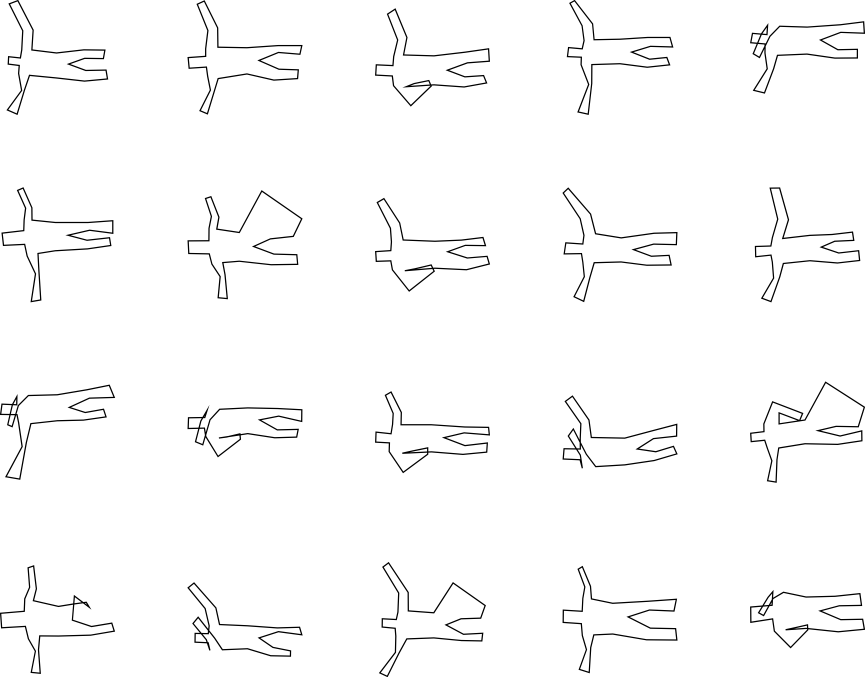
\includegraphics[width=6in]{output/3.learning/incremental/gram.19.d/samples.png}



\item Round 1\\
\label{sec-3_4_1_2}%
Here are some samples from the grammar:

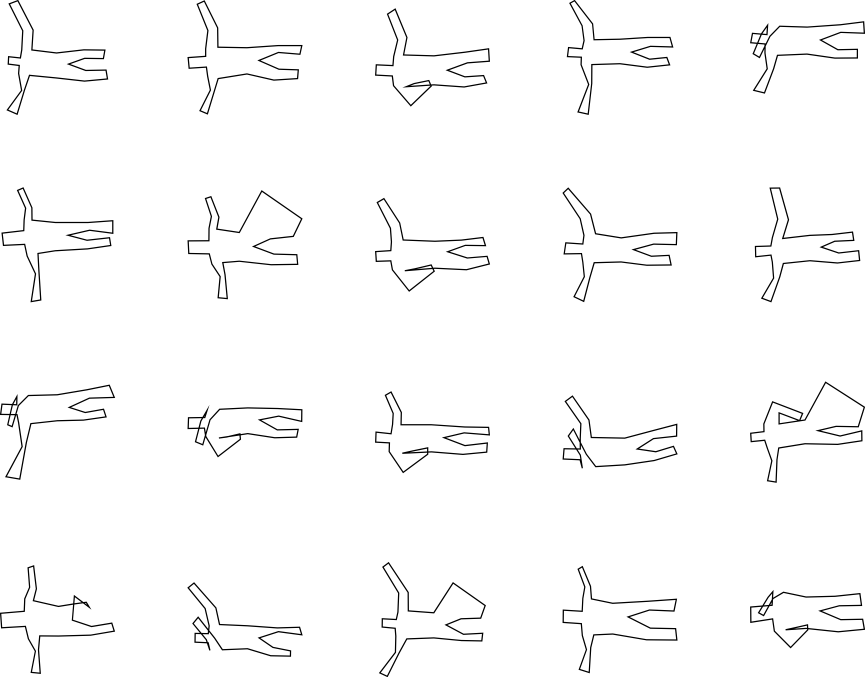
\includegraphics[width=6in]{output/3.learning/incremental/gram.19.d/samples.png}



\item Round 2\\
\label{sec-3_4_1_3}%
Here are some samples from the grammar:

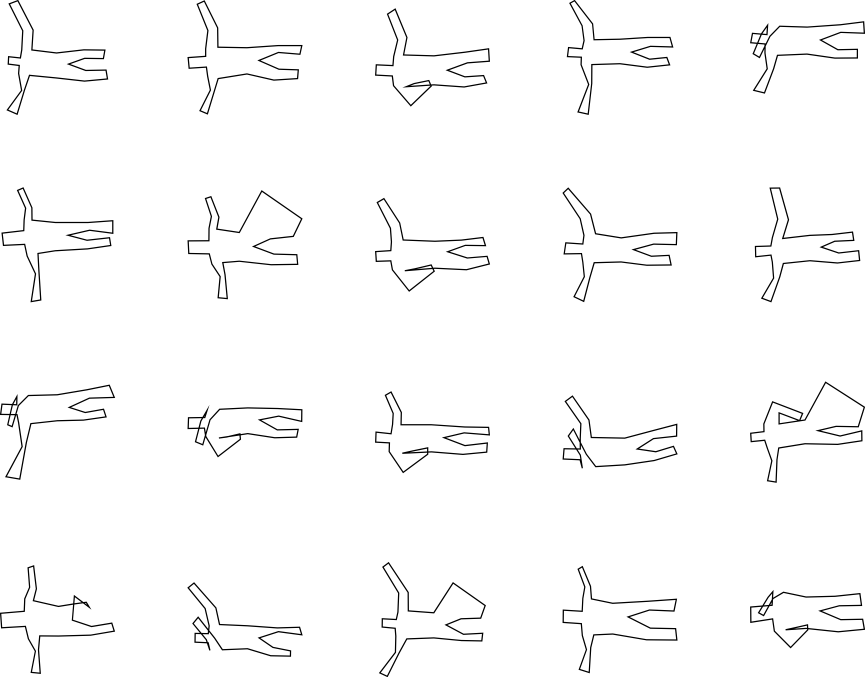
\includegraphics[width=6in]{output/3.learning/incremental/gram.19.d/samples.png}



\end{itemize} % ends low level
\subsection{Tuning with multiple midpoints, and curves of constant length}
\label{sec-3_4_2}


There may be a small bug here, since EM should settle intoa local
optimum, and the algorithm seems to be cycling between two relatively
reasonable grammars. Presumably has to do with the sparsifying
manipulations of the soft counts.

Here is our example curve, from which we build a grammar with
hand-chosen rules. We then enrich the grammar by adding in several
copies of each rule, with jittered midpoints.

%\% \#+CAPTION: Here is our example curve, from which we build a grammar
%\% \#with hand-chosen rules. We then enrich the grammar by adding in
%\% \#several copies of each rule, with jittered midpoints

\includegraphics[width=3in]{./3.em/multi_tuning/output.d/examples.eps}

Here are our training curves. We have removed one of the curves from
the training set because its correspondence to the original curve is
questionable. (It is from a frame during the flipping around of the
arm, and it is hard to pick a labeling of the points that is
consistent throughout that transition.)

%\% \#+CAPTION:    Here are our training curves:
\includegraphics[width=3in]{./3.em/multi_tuning/output.d/training.eps}
\begin{itemize}

\item Initial\\
\label{sec-3_4_2_1}%
Here are some samples from the grammar:

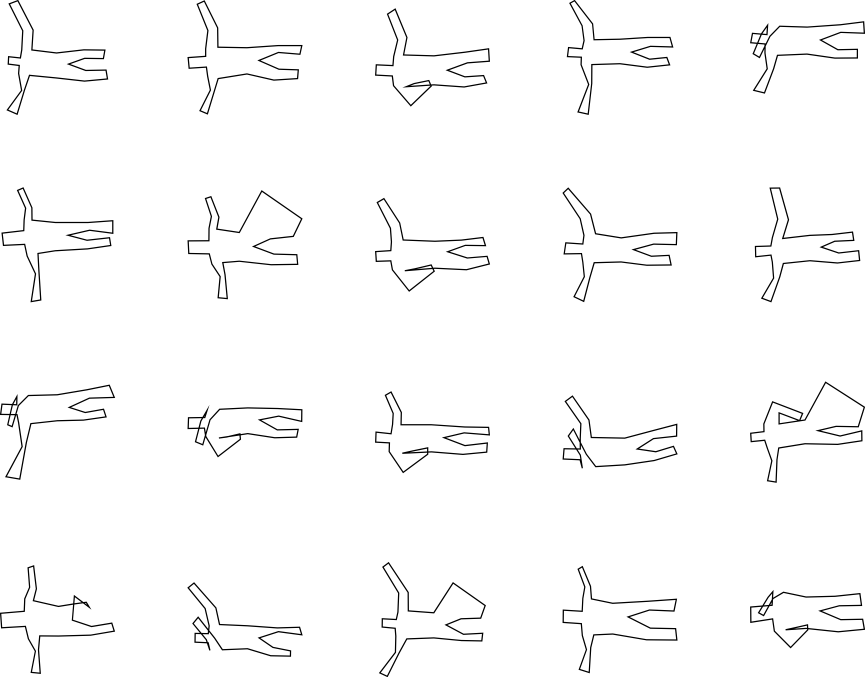
\includegraphics[width=6in]{output/3.learning/incremental/gram.19.d/samples.png}



\item Round 1\\
\label{sec-3_4_2_2}%
Here are some samples from the grammar:

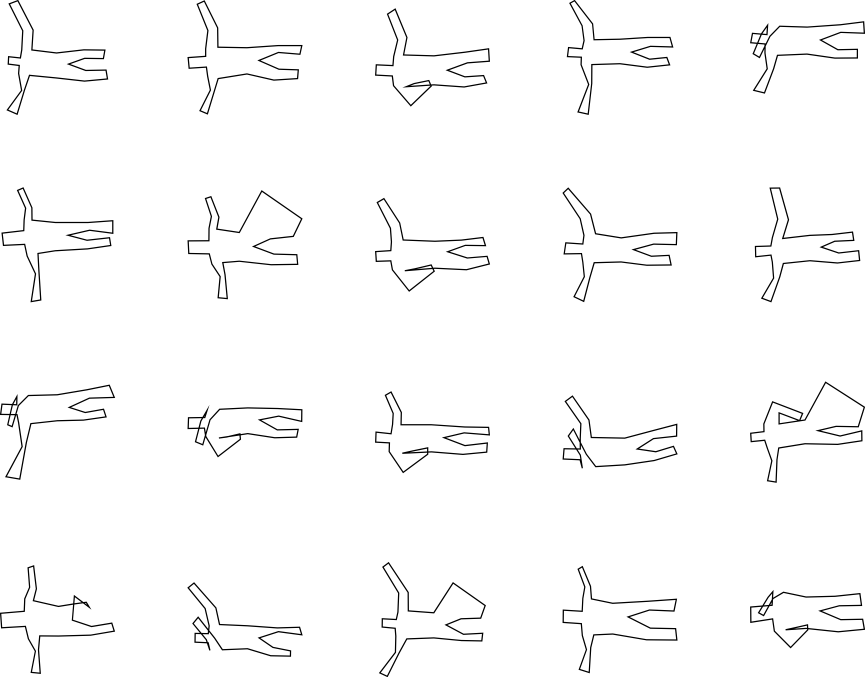
\includegraphics[width=6in]{output/3.learning/incremental/gram.19.d/samples.png}



\item Round 2\\
\label{sec-3_4_2_3}%
Here are some samples from the grammar:

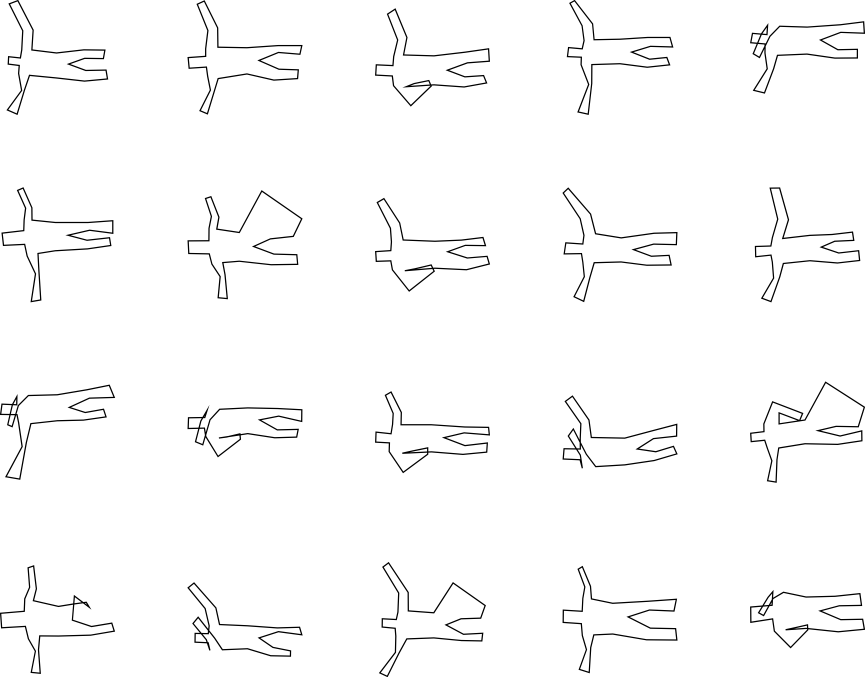
\includegraphics[width=6in]{output/3.learning/incremental/gram.19.d/samples.png}



\item Round 3\\
\label{sec-3_4_2_4}%
Here are some samples from the grammar:

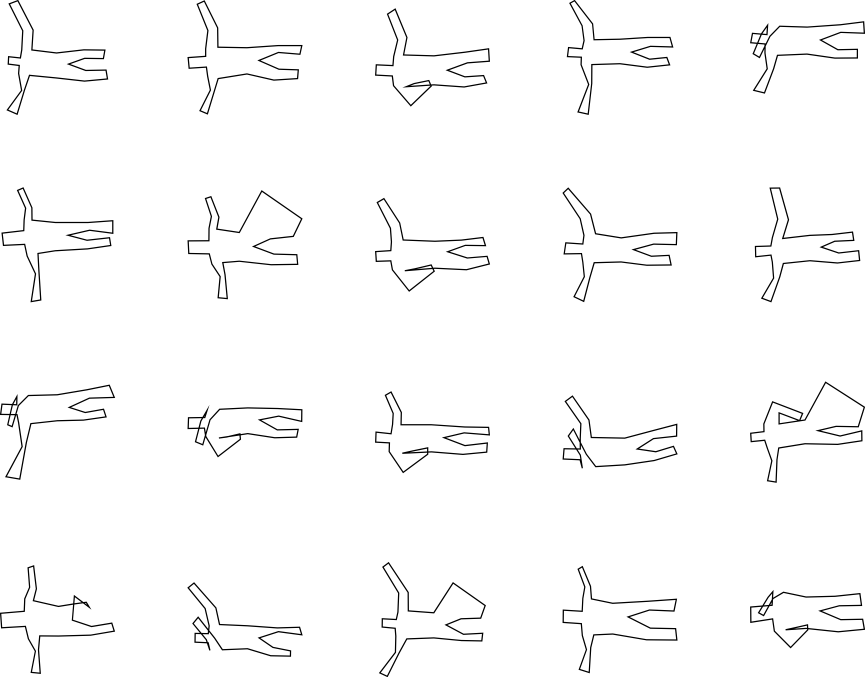
\includegraphics[width=6in]{output/3.learning/incremental/gram.19.d/samples.png}



\item Round 4\\
\label{sec-3_4_2_5}%
Here are some samples from the grammar:

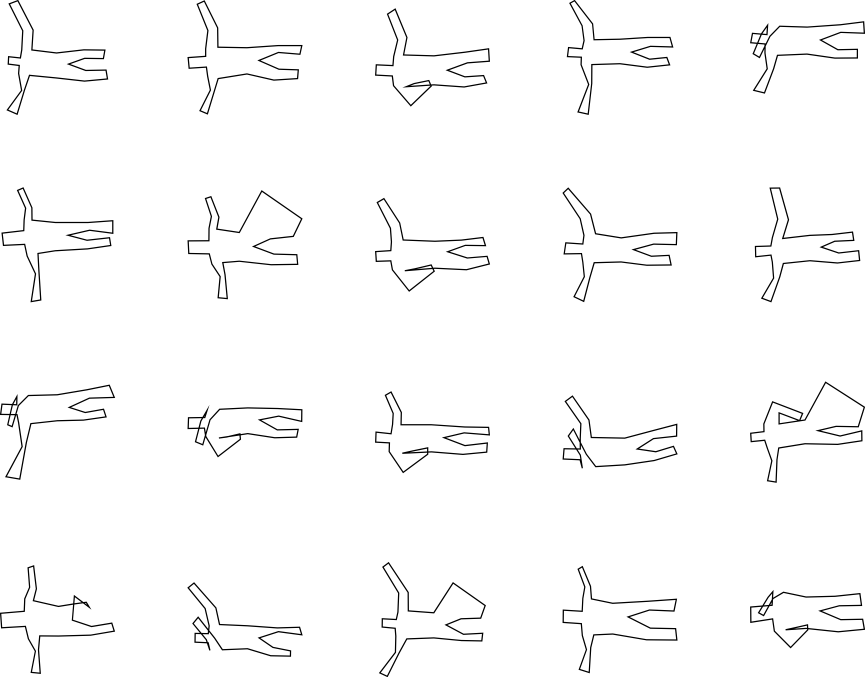
\includegraphics[width=6in]{output/3.learning/incremental/gram.19.d/samples.png}



\item Round 5\\
\label{sec-3_4_2_6}%
Here are some samples from the grammar:

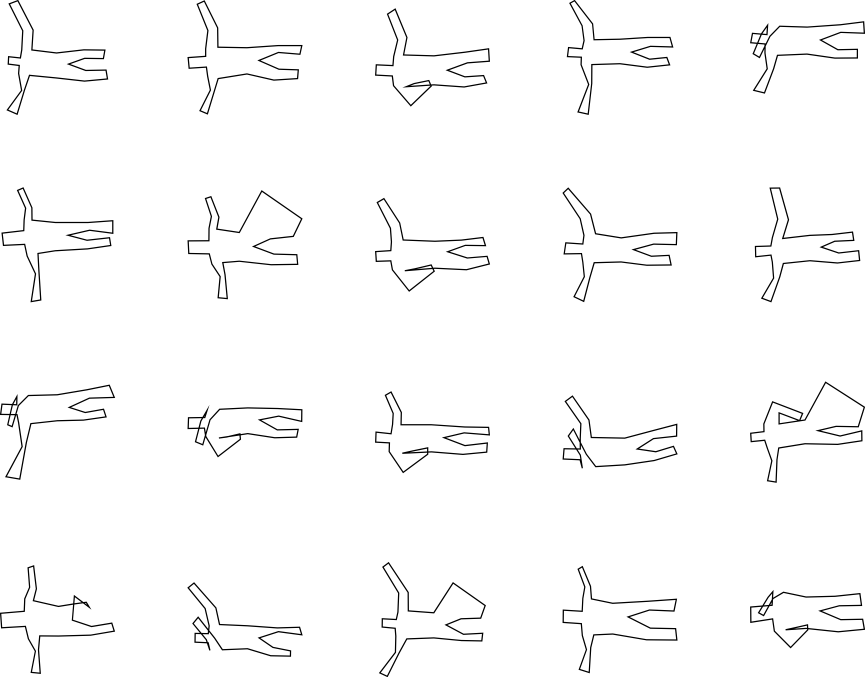
\includegraphics[width=6in]{output/3.learning/incremental/gram.19.d/samples.png}



\item Round 6\\
\label{sec-3_4_2_7}%
Here are some samples from the grammar:

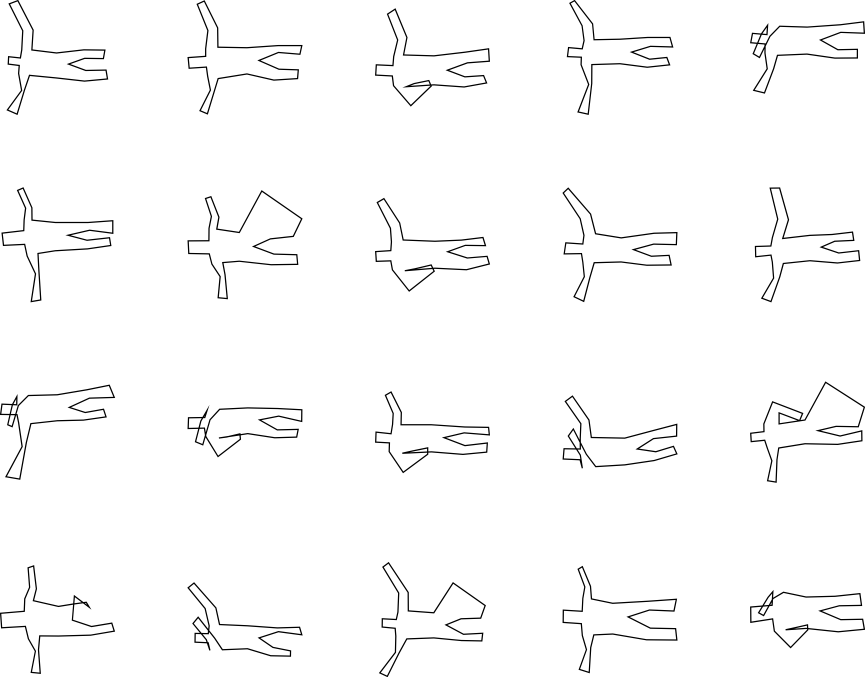
\includegraphics[width=6in]{output/3.learning/incremental/gram.19.d/samples.png}



\item Round 7\\
\label{sec-3_4_2_8}%
Here are some samples from the grammar:

\includegraphics[width=6in]{output/3.learning/incremental/gram.19.d/samples.png}



\item Round 8\\
\label{sec-3_4_2_9}%
Here are some samples from the grammar:

\includegraphics[width=6in]{output/3.learning/incremental/gram.19.d/samples.png}



\item Round 9\\
\label{sec-3_4_2_10}%
Here are some samples from the grammar:

\includegraphics[width=6in]{output/3.learning/incremental/gram.19.d/samples.png}



\item Round 10\\
\label{sec-3_4_2_11}%
Here are some samples from the grammar:

\includegraphics[width=6in]{output/3.learning/incremental/gram.19.d/samples.png}


\end{itemize} % ends low level
\subsection{Tuning with multiple midpoints, learning multi-level correlations}
\label{sec-3_4_3}


Here is the training data:

\includegraphics[width=3in]{./3.em/correlated_tuning/output.d/training.eps}
\begin{itemize}

\item Initial\\
\label{sec-3_4_3_1}%
Here are some samples from the grammar:

\includegraphics[width=6in]{output/3.learning/incremental/gram.19.d/samples.png}




\item Round 1\\
\label{sec-3_4_3_2}%
Here are some samples from the grammar:

\includegraphics[width=6in]{output/3.learning/incremental/gram.19.d/samples.png}



\item Round 2\\
\label{sec-3_4_3_3}%
Here are some samples from the grammar:

\includegraphics[width=6in]{output/3.learning/incremental/gram.19.d/samples.png}



\item Round 3\\
\label{sec-3_4_3_4}%
Here are some samples from the grammar:

\includegraphics[width=6in]{output/3.learning/incremental/gram.19.d/samples.png}



\item Round 4\\
\label{sec-3_4_3_5}%
Here are some samples from the grammar:

\includegraphics[width=6in]{output/3.learning/incremental/gram.19.d/samples.png}



\item Round 5\\
\label{sec-3_4_3_6}%
Here are some samples from the grammar:

\includegraphics[width=6in]{output/3.learning/incremental/gram.19.d/samples.png}



\item Round 6\\
\label{sec-3_4_3_7}%
Here are some samples from the grammar:

\includegraphics[width=6in]{output/3.learning/incremental/gram.19.d/samples.png}



\item Round 7\\
\label{sec-3_4_3_8}%
Here are some samples from the grammar:

\includegraphics[width=6in]{output/3.learning/incremental/gram.19.d/samples.png}



\item Round 8\\
\label{sec-3_4_3_9}%
Here are some samples from the grammar:

\includegraphics[width=6in]{output/3.learning/incremental/gram.19.d/samples.png}



\item Round 9\\
\label{sec-3_4_3_10}%
Here are some samples from the grammar:

\includegraphics[width=6in]{output/3.learning/incremental/gram.19.d/samples.png}



\item Round 10\\
\label{sec-3_4_3_11}%
Here are some samples from the grammar:

\includegraphics[width=6in]{output/3.learning/incremental/gram.19.d/samples.png}




\item Training\\
\label{sec-3_4_3_12}%
We show training data again for comparison with final samples
 
\includegraphics[width=3in]{./3.em/correlated_tuning/output.d/training.eps}

\end{itemize} % ends low level
\subsection{Adding in multiple midpoints as needed}
\label{sec-3_4_4}


Here is the training data:

\includegraphics[width=3in]{./3.em/incremental/output.d/training.eps}
\begin{itemize}

\item Initial\\
\label{sec-3_4_4_1}%
Here are some samples from the grammar:

\includegraphics[width=6in]{output/3.learning/incremental/gram.19.d/samples.png}




\item Round 1\\
\label{sec-3_4_4_2}%
Here are some samples from the grammar:

\includegraphics[width=6in]{output/3.learning/incremental/gram.19.d/samples.png}



\item Round 2\\
\label{sec-3_4_4_3}%
Here are some samples from the grammar:

\includegraphics[width=6in]{output/3.learning/incremental/gram.19.d/samples.png}



\item Round 3\\
\label{sec-3_4_4_4}%
Here are some samples from the grammar:

\includegraphics[width=6in]{output/3.learning/incremental/gram.19.d/samples.png}



\item Round 4\\
\label{sec-3_4_4_5}%
Here are some samples from the grammar:

\includegraphics[width=6in]{output/3.learning/incremental/gram.19.d/samples.png}



\item Round 5\\
\label{sec-3_4_4_6}%
Here are some samples from the grammar:

\includegraphics[width=6in]{output/3.learning/incremental/gram.19.d/samples.png}



\item Round 6\\
\label{sec-3_4_4_7}%
Here are some samples from the grammar:

\includegraphics[width=6in]{output/3.learning/incremental/gram.19.d/samples.png}



\item Round 7\\
\label{sec-3_4_4_8}%
Here are some samples from the grammar:

\includegraphics[width=6in]{output/3.learning/incremental/gram.19.d/samples.png}



\item Round 8\\
\label{sec-3_4_4_9}%
Here are some samples from the grammar:

\includegraphics[width=6in]{output/3.learning/incremental/gram.19.d/samples.png}



\item Round 9\\
\label{sec-3_4_4_10}%
Here are some samples from the grammar:

\includegraphics[width=6in]{output/3.learning/incremental/gram.19.d/samples.png}



\item Round 19\\
\label{sec-3_4_4_11}%
Here are some samples from the grammar:

\includegraphics[width=6in]{output/3.learning/incremental/gram.19.d/samples.png}




\item Round 20\\
\label{sec-3_4_4_12}%
Here are some samples from the grammar:

\includegraphics[width=6in]{output/3.learning/incremental/gram.19.d/samples.png}




\item Round 30\\
\label{sec-3_4_4_13}%
Here are some samples from the grammar:

\includegraphics[width=6in]{output/3.learning/incremental/gram.19.d/samples.png}



\item Training\\
\label{sec-3_4_4_14}%
We show training data again for comparison with final samples
 
\includegraphics[width=3in]{./3.em/incremental/output.d/training.eps}

\end{itemize} % ends low level
\section{Parsing in Cluttered Images}
\label{sec-3_5}
\subsection{Finding obvious curve}
\label{sec-3_5_1}


We build a grammar from a single curve, using a hand-picked
decomposition.

\includegraphics[width=4in]{./4.images/standard_cky/output.d/examples.eps}

We then pick some other curves which we wish to parse:

\includegraphics[width=4in]{./4.images/standard_cky/output.d/targets.eps}

We build a simple network on a 16x16 grid. We give curve segments a
data cost of 1.0, and short non-curve segments a data cost of 100.0.
On the left are the points of the network, with the curve segments
shown. On the right is the parse found.
\subsection{Fuzzy parsing}
\label{sec-3_5_2}



\begin{center}
\begin{tabular}{ll}
\hline
 \includegraphics[width=10em]{./4.images/fuzzy_cky/output.d/network.0000.eps}  &  \includegraphics[width=10em]{./4.images/fuzzy_cky/output.d/0000.yield.x8.final.eps}  \\
\hline
 \includegraphics[width=10em]{./4.images/fuzzy_cky/output.d/network.0010.eps}  &  \includegraphics[width=10em]{./4.images/fuzzy_cky/output.d/0010.yield.x8.final.eps}  \\
\hline
 \includegraphics[width=10em]{./4.images/fuzzy_cky/output.d/network.0020.eps}  &  \includegraphics[width=10em]{./4.images/fuzzy_cky/output.d/0020.yield.x8.final.eps}  \\
\hline
 \includegraphics[width=10em]{./4.images/fuzzy_cky/output.d/network.0030.eps}  &  \includegraphics[width=10em]{./4.images/fuzzy_cky/output.d/0030.yield.x8.final.eps}  \\
\hline
\end{tabular}
\end{center}




\begin{center}
\begin{tabular}{ll}
\hline
 \includegraphics[width=10em]{./4.images/fuzzy_cky/output.d/network.0040.eps}  &  \includegraphics[width=10em]{./4.images/fuzzy_cky/output.d/0040.yield.x8.final.eps}  \\
\hline
 \includegraphics[width=10em]{./4.images/fuzzy_cky/output.d/network.0050.eps}  &  \includegraphics[width=10em]{./4.images/fuzzy_cky/output.d/0050.yield.x8.final.eps}  \\
\hline
 \includegraphics[width=10em]{./4.images/fuzzy_cky/output.d/network.0060.eps}  &  \includegraphics[width=10em]{./4.images/fuzzy_cky/output.d/0060.yield.x8.final.eps}  \\
\hline
\end{tabular}
\end{center}
\subsection{Parsing actual images}
\label{sec-3_5_3}


We build a grammar using a hand-chosen annotation of this curve:
\includegraphics[width=10em]{./4.images/standard_cky/output.d/examples.eps}

Here is the image we wish to parse
\includegraphics[width=10em]{../IMG0000.eps}

Here is the set of line segments allowable during parsing. Cheaper
curves are darker red.

\includegraphics[width=10em]{./4.images/image_parsing/output.d/network.0000.eps}

Here is the curve found during parsing:

\includegraphics[width=10em]{./4.images/image_parsing/output.d/0000.yield.final.eps}
\section{Using SDF's in Other Domains}
\label{sec-3_6}
\section{Learning Structure}
\label{sec-3_7}
\subsection{Figure out optimal single-example grammar}
\label{sec-3_7_1}


We use explicit correspondences to learn the statistically best set of
constituents when building a grammar from a single example.

Note that the arms are found as constituents!

There is a strange issue here, but I've seen it before in other code
and I don't think it's a bug. Converting to Bookstein coordinates
improves the results (or here, the results are more intuitive to me),
even though the Watson distribution shouldn't need this.

Here are the constituents selected by the algorithm:

%\% \#+CAPTION:    Constituents selected.
\includegraphics[width=5in]{./6.structure/constituents/output.d/optimal.eps}

Here are the constituents that seemed most intuitive to me:

%\% \#+CAPTION:    Constituents selected.
\includegraphics[width=5in]{./6.structure/constituents/output.d/handpicked.eps}
\subsection{Constituency from approximation}
\label{sec-3_7_2}
\subsection{Constituency from decay}
\label{sec-3_7_3}


We have the following curve:

\includegraphics[width=4in]{./6.structure/constituency_heuristics/output.d/curve.eps}

We attempt to decompose the curve meaningfully by iteratively
simplifying the curve, like this:

\includegraphics[width=4in]{./6.structure/constituency_heuristics/output.d/decay.eps}


Here is the decomposition found using this heuristic.

\includegraphics[width=4in]{./6.structure/constituency_heuristics/output.d/decay_sdf.eps}
\subsection{Shock graph}
\label{sec-3_7_4}

\hyperref[==./6.structure/shock_graph/output.d/Bone-10.eps]{\# ./6.structure/shock\_graph/output.d/Bone-10.eps}
\hyperref[==./6.structure/shock_graph/output.d/Comma-10.eps]{\# ./6.structure/shock\_graph/output.d/Comma-10.eps}
\hyperref[==./6.structure/shock_graph/output.d/Glas-10.eps]{\# ./6.structure/shock\_graph/output.d/Glas-10.eps}
\hyperref[==./6.structure/shock_graph/output.d/HCircle-10.eps]{\# ./6.structure/shock\_graph/output.d/HCircle-10.eps}
\hyperref[==./6.structure/shock_graph/output.d/Heart-10.eps]{\# ./6.structure/shock\_graph/output.d/Heart-10.eps}
\hyperref[==./6.structure/shock_graph/output.d/Misk-10.eps]{\# ./6.structure/shock\_graph/output.d/Misk-10.eps}
\hyperref[==./6.structure/shock_graph/output.d/apple-10.eps]{\# ./6.structure/shock\_graph/output.d/apple-10.eps}
\hyperref[==./6.structure/shock_graph/output.d/bat-10.eps]{\# ./6.structure/shock\_graph/output.d/bat-10.eps}
%\% \#+ATTR$_{\mathrm{LATEX}}$: width=5in
%\% \includegraphics[width=10em]{./6.structure/shock_graph/output.d/beetle-10.eps}
%\% \#+ATTR$_{\mathrm{LATEX}}$: width=5in
%\% \includegraphics[width=10em]{./6.structure/shock_graph/output.d/bell-10.eps}
%\% \#+ATTR$_{\mathrm{LATEX}}$: width=5in
%\% \includegraphics[width=10em]{./6.structure/shock_graph/output.d/bird-10.eps}
%\% \#+ATTR$_{\mathrm{LATEX}}$: width=5in
%\% \includegraphics[width=10em]{./6.structure/shock_graph/output.d/bottle-10.eps}
%\% \#+ATTR$_{\mathrm{LATEX}}$: width=5in
%\% \includegraphics[width=10em]{./6.structure/shock_graph/output.d/brick-10.eps}
%\% \#+ATTR$_{\mathrm{LATEX}}$: width=5in
%\% \includegraphics[width=10em]{./6.structure/shock_graph/output.d/butterfly-10.eps}
%\% \#+ATTR$_{\mathrm{LATEX}}$: width=5in
%\% \includegraphics[width=10em]{./6.structure/shock_graph/output.d/camel-10.eps}
%\% \#+ATTR$_{\mathrm{LATEX}}$: width=5in
%\% \includegraphics[width=10em]{./6.structure/shock_graph/output.d/car-10.eps}
%\% \#+ATTR$_{\mathrm{LATEX}}$: width=5in
%\% \includegraphics[width=10em]{./6.structure/shock_graph/output.d/carriage-10.eps}
%\% \#+ATTR$_{\mathrm{LATEX}}$: width=5in
%\% \includegraphics[width=10em]{./6.structure/shock_graph/output.d/cattle-10.eps}
%\% \#+ATTR$_{\mathrm{LATEX}}$: width=5in
%\% \includegraphics[width=10em]{./6.structure/shock_graph/output.d/cellular_phone-10.eps}
%\% \#+ATTR$_{\mathrm{LATEX}}$: width=5in
%\% \includegraphics[width=10em]{./6.structure/shock_graph/output.d/chicken-10.eps}
%\% \#+ATTR$_{\mathrm{LATEX}}$: width=5in
%\% \includegraphics[width=10em]{./6.structure/shock_graph/output.d/children-10.eps}
%\% \#+ATTR$_{\mathrm{LATEX}}$: width=5in
%\% \includegraphics[width=10em]{./6.structure/shock_graph/output.d/chopper-10.eps}
%\% \#+ATTR$_{\mathrm{LATEX}}$: width=5in
%\% \includegraphics[width=10em]{./6.structure/shock_graph/output.d/classic-10.eps}
%\% \#+ATTR$_{\mathrm{LATEX}}$: width=5in
%\% \includegraphics[width=10em]{./6.structure/shock_graph/output.d/crown-10.eps}
%\% \#+ATTR$_{\mathrm{LATEX}}$: width=5in
%\% \includegraphics[width=10em]{./6.structure/shock_graph/output.d/cup-10.eps}
%\% \#+ATTR$_{\mathrm{LATEX}}$: width=5in
%\% \includegraphics[width=10em]{./6.structure/shock_graph/output.d/deer-10.eps}
%\% \#+ATTR$_{\mathrm{LATEX}}$: width=5in
%\% \includegraphics[width=10em]{./6.structure/shock_graph/output.d/device0-10.eps}
%\% \#+ATTR$_{\mathrm{LATEX}}$: width=5in
%\% \includegraphics[width=10em]{./6.structure/shock_graph/output.d/device1-10.eps}
%\% \#+ATTR$_{\mathrm{LATEX}}$: width=5in
%\% \includegraphics[width=10em]{./6.structure/shock_graph/output.d/device2-10.eps}
%\% \#+ATTR$_{\mathrm{LATEX}}$: width=5in
%\% \includegraphics[width=10em]{./6.structure/shock_graph/output.d/device3-10.eps}
%\% \#+ATTR$_{\mathrm{LATEX}}$: width=5in
%\% \includegraphics[width=10em]{./6.structure/shock_graph/output.d/device4-10.eps}
%\% \#+ATTR$_{\mathrm{LATEX}}$: width=5in
%\% \includegraphics[width=10em]{./6.structure/shock_graph/output.d/device5-10.eps}
%\% \#+ATTR$_{\mathrm{LATEX}}$: width=5in
%\% \includegraphics[width=10em]{./6.structure/shock_graph/output.d/device6-10.eps}
%\% \#+ATTR$_{\mathrm{LATEX}}$: width=5in
%\% \includegraphics[width=10em]{./6.structure/shock_graph/output.d/device7-10.eps}
%\% \#+ATTR$_{\mathrm{LATEX}}$: width=5in
%\% \includegraphics[width=10em]{./6.structure/shock_graph/output.d/device8-10.eps}
%\% \#+ATTR$_{\mathrm{LATEX}}$: width=5in
%\% \includegraphics[width=10em]{./6.structure/shock_graph/output.d/device9-10.eps}
%\% \#+ATTR$_{\mathrm{LATEX}}$: width=5in
%\% \includegraphics[width=10em]{./6.structure/shock_graph/output.d/dog-10.eps}
%\% \#+ATTR$_{\mathrm{LATEX}}$: width=5in
%\% \includegraphics[width=10em]{./6.structure/shock_graph/output.d/elephant-10.eps}
%\% \#+ATTR$_{\mathrm{LATEX}}$: width=5in
%\% \includegraphics[width=10em]{./6.structure/shock_graph/output.d/face-10.eps}
%\% \#+ATTR$_{\mathrm{LATEX}}$: width=5in
%\% \includegraphics[width=10em]{./6.structure/shock_graph/output.d/fish-10.eps}
%\% \#+ATTR$_{\mathrm{LATEX}}$: width=5in
%\% \includegraphics[width=10em]{./6.structure/shock_graph/output.d/flatfish-10.eps}
%\% \#+ATTR$_{\mathrm{LATEX}}$: width=5in
%\% \includegraphics[width=10em]{./6.structure/shock_graph/output.d/fly-10.eps}
%\% \#+ATTR$_{\mathrm{LATEX}}$: width=5in
%\% \includegraphics[width=10em]{./6.structure/shock_graph/output.d/fork-10.eps}
%\% \#+ATTR$_{\mathrm{LATEX}}$: width=5in
%\% \includegraphics[width=10em]{./6.structure/shock_graph/output.d/fountain-10.eps}
%\% \#+ATTR$_{\mathrm{LATEX}}$: width=5in
%\% \includegraphics[width=10em]{./6.structure/shock_graph/output.d/frog-10.eps}
%\% \#+ATTR$_{\mathrm{LATEX}}$: width=5in
%\% \includegraphics[width=10em]{./6.structure/shock_graph/output.d/guitar-10.eps}
%\% \#+ATTR$_{\mathrm{LATEX}}$: width=5in
%\% \includegraphics[width=10em]{./6.structure/shock_graph/output.d/hammer-10.eps}
%\% \#+ATTR$_{\mathrm{LATEX}}$: width=5in
%\% \includegraphics[width=10em]{./6.structure/shock_graph/output.d/hat-10.eps}
%\% \#+ATTR$_{\mathrm{LATEX}}$: width=5in
%\% \includegraphics[width=10em]{./6.structure/shock_graph/output.d/horse-10.eps}
%\% \#+ATTR$_{\mathrm{LATEX}}$: width=5in
%\% \includegraphics[width=10em]{./6.structure/shock_graph/output.d/horseshoe-10.eps}
%\% \#+ATTR$_{\mathrm{LATEX}}$: width=5in
%\% \includegraphics[width=10em]{./6.structure/shock_graph/output.d/jar-10.eps}
%\% \#+ATTR$_{\mathrm{LATEX}}$: width=5in
%\% \includegraphics[width=10em]{./6.structure/shock_graph/output.d/key-10.eps}
%\% \#+ATTR$_{\mathrm{LATEX}}$: width=5in
%\% \includegraphics[width=10em]{./6.structure/shock_graph/output.d/lizzard-10.eps}
%\% \#+ATTR$_{\mathrm{LATEX}}$: width=5in
%\% \includegraphics[width=10em]{./6.structure/shock_graph/output.d/lmfish-10.eps}
%\% \#+ATTR$_{\mathrm{LATEX}}$: width=5in
%\% \includegraphics[width=10em]{./6.structure/shock_graph/output.d/octopus-10.eps}
%\% \#+ATTR$_{\mathrm{LATEX}}$: width=5in
%\% \includegraphics[width=10em]{./6.structure/shock_graph/output.d/pencil-10.eps}
%\% \#+ATTR$_{\mathrm{LATEX}}$: width=5in
%\% \includegraphics[width=10em]{./6.structure/shock_graph/output.d/personal_car-10.eps}
%\% \#+ATTR$_{\mathrm{LATEX}}$: width=5in
%\% \includegraphics[width=10em]{./6.structure/shock_graph/output.d/pocket-10.eps}
%\% \#+ATTR$_{\mathrm{LATEX}}$: width=5in
%\% \includegraphics[width=10em]{./6.structure/shock_graph/output.d/rat-10.eps}
%\% \#+ATTR$_{\mathrm{LATEX}}$: width=5in
%\% \includegraphics[width=10em]{./6.structure/shock_graph/output.d/ray-10.eps}
%\% \#+ATTR$_{\mathrm{LATEX}}$: width=5in
%\% \includegraphics[width=10em]{./6.structure/shock_graph/output.d/sea_snake-10.eps}
%\% \#+ATTR$_{\mathrm{LATEX}}$: width=5in
%\% \includegraphics[width=10em]{./6.structure/shock_graph/output.d/shoe-10.eps}
%\% \#+ATTR$_{\mathrm{LATEX}}$: width=5in
%\% \includegraphics[width=10em]{./6.structure/shock_graph/output.d/spoon-10.eps}
%\% \#+ATTR$_{\mathrm{LATEX}}$: width=5in
%\% \includegraphics[width=10em]{./6.structure/shock_graph/output.d/spring-10.eps}
%\% \#+ATTR$_{\mathrm{LATEX}}$: width=5in
%\% \includegraphics[width=10em]{./6.structure/shock_graph/output.d/stef-10.eps}
%\% \#+ATTR$_{\mathrm{LATEX}}$: width=5in
%\% \includegraphics[width=10em]{./6.structure/shock_graph/output.d/teddy-10.eps}
%\% \#+ATTR$_{\mathrm{LATEX}}$: width=5in
%\% \includegraphics[width=10em]{./6.structure/shock_graph/output.d/tree-10.eps}
%\% \#+ATTR$_{\mathrm{LATEX}}$: width=5in
%\% \includegraphics[width=10em]{./6.structure/shock_graph/output.d/truck-10.eps}
%\% \#+ATTR$_{\mathrm{LATEX}}$: width=5in
%\% \includegraphics[width=10em]{./6.structure/shock_graph/output.d/turtle-10.eps}
%\% \#+ATTR$_{\mathrm{LATEX}}$: width=5in
%\% \includegraphics[width=10em]{./6.structure/shock_graph/output.d/watch-10.eps}
\section{Learning Texture}
\label{sec-3_8}
\subsection{Trying to learn a texture-only grammar}
\label{sec-3_8_1}

\begin{itemize}
\item set up some hierarchy of scales, with decompositions between them

\begin{itemize}
\item would like to use all the data we can get, which means we want
      every length of curve to be close to some scale
\end{itemize}

\item build a grammar from this
\item learn midpoint distributions by going over all pairs of curve
    points and taking the midpoint (and maybe other percentiles) by
    arclength to get triangles
\item sample from it
\item Here are samples from such a grammar, built from every class of
    the Swedish leaf dataset. Some classes are being modeled
    reasonably, some are not.
\end{itemize}
\begin{itemize}

\item Class 1\\
\label{sec-3_8_1_1}%
Training:

\includegraphics[width=4in]{./7.texture/scaled_nts/output.d/scaled_nts_training.1.eps}

Samples:

\includegraphics[width=4in]{./7.texture/scaled_nts/output.d/scaled_nts.1.eps}


\item Class 2\\
\label{sec-3_8_1_2}%
Training:

\includegraphics[width=4in]{./7.texture/scaled_nts/output.d/scaled_nts_training.2.eps}

Samples:

\includegraphics[width=4in]{./7.texture/scaled_nts/output.d/scaled_nts.2.eps}


\item Class 3\\
\label{sec-3_8_1_3}%
Training:

\includegraphics[width=4in]{./7.texture/scaled_nts/output.d/scaled_nts_training.3.eps}

Samples:

\includegraphics[width=4in]{./7.texture/scaled_nts/output.d/scaled_nts.3.eps}


\item Class 4\\
\label{sec-3_8_1_4}%
Training:

\includegraphics[width=4in]{./7.texture/scaled_nts/output.d/scaled_nts_training.4.eps}

Samples:

\includegraphics[width=4in]{./7.texture/scaled_nts/output.d/scaled_nts.4.eps}


\item Class 5\\
\label{sec-3_8_1_5}%
Training:

\includegraphics[width=4in]{./7.texture/scaled_nts/output.d/scaled_nts_training.5.eps}

Samples:

\includegraphics[width=4in]{./7.texture/scaled_nts/output.d/scaled_nts.5.eps}


\item Class 6\\
\label{sec-3_8_1_6}%
Training:

\includegraphics[width=4in]{./7.texture/scaled_nts/output.d/scaled_nts_training.6.eps}

Samples:

\includegraphics[width=4in]{./7.texture/scaled_nts/output.d/scaled_nts.6.eps}


\item Class 7\\
\label{sec-3_8_1_7}%
Training:

\includegraphics[width=4in]{./7.texture/scaled_nts/output.d/scaled_nts_training.7.eps}

Samples:

\includegraphics[width=4in]{./7.texture/scaled_nts/output.d/scaled_nts.7.eps}


\item Class 8\\
\label{sec-3_8_1_8}%
Training:

\includegraphics[width=4in]{./7.texture/scaled_nts/output.d/scaled_nts_training.8.eps}

Samples:

\includegraphics[width=4in]{./7.texture/scaled_nts/output.d/scaled_nts.8.eps}


\item Class 9\\
\label{sec-3_8_1_9}%
Training:

\includegraphics[width=4in]{./7.texture/scaled_nts/output.d/scaled_nts_training.9.eps}

Samples:

\includegraphics[width=4in]{./7.texture/scaled_nts/output.d/scaled_nts.9.eps}


\item Class 10\\
\label{sec-3_8_1_10}%
Training:

\includegraphics[width=4in]{./7.texture/scaled_nts/output.d/scaled_nts_training.10.eps}

Samples:

\includegraphics[width=4in]{./7.texture/scaled_nts/output.d/scaled_nts.10.eps}


\item Class 11\\
\label{sec-3_8_1_11}%
Training:

\includegraphics[width=4in]{./7.texture/scaled_nts/output.d/scaled_nts_training.11.eps}

Samples:

\includegraphics[width=4in]{./7.texture/scaled_nts/output.d/scaled_nts.11.eps}


\item Class 12\\
\label{sec-3_8_1_12}%
Training:

\includegraphics[width=4in]{./7.texture/scaled_nts/output.d/scaled_nts_training.12.eps}

Samples:

\includegraphics[width=4in]{./7.texture/scaled_nts/output.d/scaled_nts.12.eps}


\item Class 13\\
\label{sec-3_8_1_13}%
Training:

\includegraphics[width=4in]{./7.texture/scaled_nts/output.d/scaled_nts_training.13.eps}

Samples:

\includegraphics[width=4in]{./7.texture/scaled_nts/output.d/scaled_nts.13.eps}


\item Class 14\\
\label{sec-3_8_1_14}%
Training:

\includegraphics[width=4in]{./7.texture/scaled_nts/output.d/scaled_nts_training.14.eps}

Samples:

\includegraphics[width=4in]{./7.texture/scaled_nts/output.d/scaled_nts.14.eps}


\item Class 15\\
\label{sec-3_8_1_15}%
Training:

\includegraphics[width=4in]{./7.texture/scaled_nts/output.d/scaled_nts_training.15.eps}

Samples:

\includegraphics[width=4in]{./7.texture/scaled_nts/output.d/scaled_nts.15.eps}



\end{itemize} % ends low level
\chapter{Working notes - new front burner (limit 5, each should fit on one emacs page)}
\label{sec-4}
\section{Shock graphs and adaptive SDF's to get good constituents}
\label{sec-4_1}

\begin{itemize}
\item getting somewhat OK constituents, but getting far too many very
    similar ones
\item probably want to incorporate information from the outside skeleton
    at some point, but it's unclear how to mix the two (maybe we don't
    have to do anything, can just mix the two)
\item setting the threshold to -5 makes it crash on the spoon, should
    figure that out
\item having a lot of trouble with markov-style rules. it seems like
    this is kind of a weakness of shock graphs in general. how do we
    defeat it?

\begin{itemize}
\item deleting vertices of degree 2 helps some, but there are cases
      where we don't want to do that.
\item some markov-style rules come from singleton branches. how do we
      detect those???
\end{itemize}

\end{itemize}
\section{2D parsing}
\label{sec-4_2}

\begin{itemize}
\item datacosts

\begin{itemize}
\item seemed to be workign somewhat OK, thresholding was not doing well though
\end{itemize}

\item low-level curves available

\begin{itemize}
\item currently i believe we are just thresholding
\item we were thinking about a thinning strategy, it seemed somewhat reasonable?
\end{itemize}

\item search strategy

\begin{itemize}
\item standard CKY is on the edge of acceptability, depending on how
      sparse the set of curves is
\item we had fuzzy$_{\mathrm{cky}}$, which worked sort of ok but was probably too messy
\item we came up with an elaborate multipass strategy that should
      optimize the same thing as standard cky, except that it had
      trouble with d(p,r) < d(p,q), d(q,r)
\end{itemize}

\end{itemize}
\section{Discriminative EM}
\label{sec-4_3}

\begin{itemize}
\item subsample the leaves to be smallish
\item make a niceish sdf with bottom$_{\mathrm{out}}$ function
\item make the initial grammars
\item get the viterbi parses and/or soft counts
\item make a vector with on entry for every X->l rule and one entry for every midpoint
\item write an svm

\begin{itemize}
\item use stochastic gradient descent, pedro thinks it should work
\item give it some reasonably separable dataset from bishop or something to test
\end{itemize}

\end{itemize}
\chapter{Working notes - front burner (limit 5)}
\label{sec-5}
\section{Adaptive SDF's}
\label{sec-5_1}


\begin{itemize}
\item Next step: unfuck the subsampling code to the point where it will
    give us an intelligent subsampling that has like 8-10 points.

    easiest is to search on a trellis so that we know exactly how long
    the curve is that we are constructing. then we can pick the one we
    like best among the available lengths. This will run in time tl,
    where t is old time and l is max length. Therefore, we want to
    limit it to the last iteration or so.

    this is kind of hard to think about. how do we know what length we
    want? some curves are just more open to being approximated by
    fewer lines.

    in fact, this seems like a bad idea. We should just construct the
    full family on the coarsest curve. If we want to have fewer
    compositions there, we will just have to do it with constituency
    heuristics
\item can just have the subsampler call itself again with a higher
    regularization weight if it is above a hard maximum length
\item That's still 8*7*6/2 \~{} 160. But if we require balance etc. it
    might get lower than that. Coding it is the easiest way to find out.
\item do several iterations of subsampling
\item we wrote down a rule in the notebook that keeps the family
    $\theta$-flexible
\item need to figure out what to do with the top-level, it still has 18
    points. Can we actually have that many rules? it would be
    18*17*16? Certainly at least that over 6, which is about 800,
    probably that over 2, about 2400
\item the subsampling algorithm doesn't want to make the curve much coarser
\end{itemize}
\begin{itemize}
\item can decrease the number of rules slightly be only looking at
    relatively balanced ones, that won't exclude many reasonable
    parses
\item for every sub-interval of the top-level, it is either short or
    long. For the long ones, we can add its rules now.
\item For short intervals at the top level, we remember them and use
    them as seeds for the next level
\item At the next level, look at every seed. Sub-intervals of these
    seeds are allowable intervals now. Iterate over all sub-intervals
    of every seed. If they are long enough, add rules now. Otherwise,
    make them seeds for the next level.
\item Try parsing a full Romer curve with the hand-built Romer. Good
    test because it needs to have very good constituents and it needs
    to be very efficient.
\item can we tie the cost function to the original curve throughout, or
    will it be tied to the current approximation? More important for
    length balance terms than data terms, probably
\end{itemize}
\section{2D approximate parsing}
\label{sec-5_2}


\begin{itemize}
\item thoughts on the curve network

\begin{itemize}
\item we want a curve network that contains some representative of
      every reasonable segment, but that doesn't have many
      representatives of each (i.e., nms). We also want to make sure
      that every pair of reasonable curves C$_{\mathrm{pq}}$, C$_{\mathrm{qr}}$ has a
      representative pair C$_p$'q', C$_q$'r', so that we do not lose any
      compositions. If we have both of those things, we should be OK
      during parsing.
\item Make a list of all line segments which have some evidence under
      them.
\item Remove C$_{\mathrm{pq}}$ if there is a nearby segment C$_{\mathrm{pq}}$' which has more
      evidence, and such that, for every C$_{\mathrm{qr}}$, there is a C$_q$'r which
      has more evidence than C$_{\mathrm{qr}}$, with q\~{}q'. Might be sufficient if
      there is a C$_q$'r for which C$_{\mathrm{pq}}$', C$_q$'r together have more
      evidence than C$_{\mathrm{pq}}$, C$_{\mathrm{qr}}$ together, with q\~{}q'.

      Question: Do we have to fix p? Imagine taking our favorite curve
      and trying to prove that it was not thrown out. We can move any
      one point q by considering p,r on either side of it, and finding
      the relevant q' such that C$_{\mathrm{pq}}$', C$_q$'r were preserved. 

      But then we want to fix both p and q\ldots{}

      i thought of a way out of this, just have to remember. involved
      thinking of the curve evolving over time as we remove things, as
      long as we can always move the curve to something that still
      exists, is close, and has better qual, then we're OK

      could think of just queuing everything up and somehow counting
      references or otherwise making sure we have what we want
\end{itemize}

\item How do we make a better curve network for an image? This sounds promising:

\begin{itemize}
\item take gradients, calculate costs as now
\item look at (avg$_{\mathrm{gradient}}$*length + A)/length as a way to reward
      longness, and pick the single best curve
\item using the current data functions, make that curve and a few
      longer and shorter versions of it
\item remove the gradient near that curve. Should probably leave it
      near the endpoints. HOW do we remove gradient? We want to be
      fairly agressive about it, but we also want to avoid deleting
      data necessary for compositions. We could mask the gradient
      images, so that we don't see used data while choosing the next
      curve, but do still see it when we actually compute the cost of
      the segment.
\item How do we mask based on C$_{\mathrm{pq}}$? First, chop off 10-20\% on each
      side. Then, round each remaining point to the grid. Then, return
      0 on future gradient queries at (x,y) if (x,y) rounds to the
      same grid point.
\item need large while loop.
\item consider relaxing the angle requirement
\end{itemize}

\item We need to break the link between the network and the parsing
    paradigm. This means separate executables, one that makes the
    network and one that reads it in. That will make the code much
    easier to maintain and adapt. It should be easy:

\begin{itemize}
\item construct the net, save network image, save edge file
\item load the net
\item could even have a separate noise-adding function
\end{itemize}

\item Going from easier versions to hard versions:

\begin{itemize}
\item how much geometric variation is there?

      Can add a ton of geometric variation by simply iterating over
      Romer curves.
\item how many extra fake edges are there?

      We can add 10? random edges. We should pick edges that are
      relatively short, that is most realistic and most confusing

      To be most brutal, we can independently set the cost of each
      default edge from a distribution that has a tiny bit of weight
      at cost 1.0, and set the cost of each true edge from a
      distribution that has some weight at costs higher than 1.0, and
      include default edges at scales that include the scales of the
      true edges, the longest of which has length 9. (But we can
      probably say that the larger scales have a lower false positive
      rate for edge detectors?)

      OK, now it takes 40 minutes and the results are
      garbage. Probably not that bad a sign, since the input looks
      super bad.

      If we can do reasonably on this, we are ready to run on images.

      how do we run on images? We need a cost for each line
      segment. we could just get a canny pyramid and round the line
      segment. Or we could just run canny on it, and then count the
      number of edge pixels with the right one of 8 (4?) orientations

      we could do canny, round orientations, spread slightly, and then
      simply take the average value under the segment. that seems
      cleanest. Scale shouldn't matter because it's an average, the
      spreading should make it relatively robust.

      we want cheapness to be good, so what should we do with
      gradient? Could do 1/(1+gradmag), that has an upper bound on the
      cost and dies off relatively slowly as gradient builds up. Need
      to think about weighting of data vs. geometry, obviously. 

      the grid is trimming the image a bit too much. Should round the
      image size up to the next multiple of granularity by copying
      border pixels

      not working at all. try taking absolute value after summing.

      big problem - a segment has high gradient/low cost if it is 45
      degrees off of the correct direction, which is no good at
      all. We only actually want it to have low gradient if it is very
      close to the correct angle. We can get the sine of the angle
      between gradient and segment for each pixel. We should just give
      no gradient if the angle is off by more than a bit

      Before we do that, we should start running in parallel, because
      this will slow it way the fuck down.

      OK, it's failing utterly, but it's obvious why. Since we don't
      allow any structural variation, not even L->LL, and since we
      only include default edges of length <= 3, the long missing
      segments are simply impossible to create. Think about it, should
      be easy to fix\ldots{}
\item how many true edges are missing?

      We can fail to add the true curve edges in with some probability.
\end{itemize}

\item Speed: takes 181 minutes / 3 hours to run on 16 images with 32x32
    grid and maxlen=8. This is about 11-12 minutes per image.

    That's relatively slow. Running 16x16 standard takes 3 minutes,
    for comparison. Running 32x32 would presumably take 24 minutes.

    Could start running these in parallel. Can do in python?
\item We have a hierarchy of grids, similar to an image pyramid.

    We have curves between each pair of points. (Really they specify
    only the beginning and end of the curve, not the behavior in
    between.)

    We can compose two curves C$_{\mathrm{pq}}$, C$_{\mathrm{qr}}$ to get another curve, C$_{\mathrm{pr}}$.

    Unfortunately, the number of curves and compositions is
    prohibitively high (N$^2$=n$^4$ and N$^3$=n$^6$, respectively, where we
    have a grid of size nxn with N points), and we would like to use a
    restricted subset of them as a proxy for the full set.

    We would like it to be the case that any parse tree over the full
    set can be modified very slightly to be over the restricted
    subset.

    There are many issues with this.
\item Our current strategy is as follows: we allow only curves of length
    <= maxlen * (current side length of grid square). Currently we are
    using maxlen=8.

    We parse by starting at the finest grid, looking for compositions
    in the current grid, and then lifting P(X$\to$ C$_{\mathrm{pq}}$) up to the next
    coarser grid by rounding p and q to the next coarser
    grid. Terminal line segments are inserted at the beginning of
    parsing without regard to their length, so they will be lifted up
    along with everything else until the grid is coarse enough for them.

    We only lift C$_{\mathrm{pq}}$ when d(p,q) is at least the step size of the new
    grid. Unsure if that is the right idea.
\item How much can the segment pq be deformed by the lifting process,
    especially given that we lift the same thing repeatedly? We can
    say the following: let pq be a segment, and G be any rectangular
    subset of the grid that is aligned to coarse grid points at level
    i. If p lies inside of G initially, then even after rounding it
    will always lie inside of G. If p lies outside of G initially,
    then rounding it can push it to lie on the boundary of G, but can
    never push it to lie in the interior of G.

    This gives us some lower bound on the length distortion. If d(p,q)
    is larger than 1.414*gridlength$_i$, then p and q must lie in
    different grid squares, and they will not be collapsed together by
    rounding to level i.
\item We should almost certainly use the trick of making the maxlen
    longer as we go up. Think about that, it's probably not so bad. It
    means we can terminate safely sooner, which we should think about.

    Q: when can we stop?
\item If we switched to a more direct for-loop over the grid, we could
    potentially save a lot of computation by restricting to the maxlen
    linf-neighborhood.
\item Notes on visualizing parses:

\begin{itemize}
\item It might be good to color the segments by their grid level,
      rather than their depth in the parse tree (although we can
      always look up either)
\item drawing is imperfect, because a segment can be covered up by its
      cousin in a righter subtree. Only way to ensure that
      highest-level color is used is to make a list sorted by rank and
      then do it. Since we know the depth, we could be inserting into
      lists, so it wouldn't be hard at all. Might also be good to
      label each segment as belonging to whichever levels it belongs
      to, and then commingling the colors, so that we know \textbf{all} the
      levels.
\end{itemize}

\item A much riskier optimization is to drop parse table entries that
    are high relative to other comparable entries. this could save a
    \textbf{huge} amount of time, but it would be easy to get rid of
    necessary pieces. 

    One interesting idea: suppose we throw out X$\to$ C$_{\mathrm{pq}}$ when its cost
    is above a threshold T, say 100 times the cheapest cost of X$\to$
    C$_{\mathrm{xy}}$, or 100 more than the cheapest cost. Then, suppose that
    future queries to cost(X$\to$ C$_{\mathrm{pq}}$) have maximum cost T, rather than
    infinity. This would not actually get rid of any parses, since we
    would essentially assume the existence of any parse that could
    have been dropped. The one issue is that we can then no longer
    skip X$\to$ YZ, Y$\to$ C$_{\mathrm{pq}}$ if cost(Y$\to$ C$_{\mathrm{pq}}$) is infinity. But, we
    might get some amount of the same effect if we check whether
    cost(Y$\to$ C$_{\mathrm{pq}}$) > T$_X$. If the factor 100 was instead set somewhat
    adaptively, so that it got lower as we went up, then we would be
    OK, because when cost(Y$\to$ C$_{\mathrm{pq}}$) is infinity in the current model,
    it would instead be T$_Y$, and if T$_Y$ > T$_X$, we would be good. We
    would need to work out some sort of threshold schedule such that
    we would usually get that savings.

    Suppose that the factor is an additive A$_X$ (in the log domain)
    rather than multiplicative. Then we would like it to usually be
    the case that

      T$_X$ < T$_Y$

    which means we need

      bestcost(X) + A$_X$ < bestcost(Y) + A$_Y$, 

    even though cost(X) = cost(Y) + cost(Z) + geometry. So in
    particular, we would need that bestcost(Z) + geometry + A$_X$ < A$_Y$
    most of the time.

    What if we did multiple passes with different A$_X$, but used
    infinity as the default value instead of T$_Y$? The advantage of
    this is that we are finding true parses, so we are building up
    legitimate values of bestcost, which gives us a much better idea
    of how strict to be.
    
    Alternatively, we can ask for the bestcost in a restricted
    region. Clearly we can discard something if it is not the best in
    a trivial region including only itself. Clearly doing this
    globally could prevent something useful from being found. What if
    we do it with a k x k breakdown of the points? We are probably
    just replicating the fuzzy algorithm at that point.

    What if we change the algorithm to be coarse to fine somehow? We
    run parsing from fine to coarse as we do now, but we start at a
    relatively coarse level the first time, and then repeat it with
    finer and finer levels.

    The point is that we can potentially skip looking at X$\to$ C$_{\mathrm{pr}}$ if
    we have a lower bound on the cost, which the previous iteration
    should give us (modulo the shape costs being slightly inaccurate)

    One problem with this idea is that we iterate over p,q first
    instead of p,r.

    We could say that when looking at X$\to$ YZ, we skip Y$\to$ C$_{\mathrm{pq}}$ if
    its cost at the current pass is more than the maximum cost of X$\to$
    C$_{\mathrm{pr}}$ (over reachable r) at the previous pass. So it could not
    improve on any parse that we know about, and in the coarse-to-fine
    world we would (hopefully?) know about every parse. (We would have
    to be sure to lift \textbf{all} the segments when doing coarser
    passes. It seems like it might be important to get stuff that
    would have have length 0, because it would allow us to actually
    always see the true curve.)

    As a slight modification of the above, we could use, instead of
    max$_r$ cost(X$\to$ C$_{\mathrm{pr}}$), min$_r$ cost(X$\to$ C$_{\mathrm{pr}}$) + buffer. This on the
    theory that good parses are very sparse, so max$_r$ cost(X$\to$ C$_{\mathrm{pr}}$)
    will always be extremely high and basically meaningless. We would
    be assuming that the true parse would pass this test, but it
    doesn't seem that bad. Since p is fixed, we're not considering
    everything, so we will only be tricked if this subset of the true
    parse is close to a place where this subset fits \textbf{much}
    better. (Depending on buffer, obviously.)

    This sounds pretty cool but is slightly too complicated for
    now. It can be one of the next things we try, though, since
    speeding it up is important.

    More thoughts on ctf fuzzy: when we are searching over the first
    two points p,q, arguably the most relevant quantity is how good of
    a \textbf{context} exists for X$\to$ C$_{\mathrm{pq}}$. Thus if we have a lower bound on
    the ``outside cost'' of a parse tree containing X$\to$ C$_{\mathrm{pq}}$, we know
    whether we are interested in X$\to$ C$_{\mathrm{pq}}$. If cost(X$\to$ C$_{\mathrm{pq}}$) +
    lboutside(X$\to$ C$_{\mathrm{pq}}$) > bestparsequality, then we can safely ignore
    X$\to$ C$_{\mathrm{pq}}$.

    How do we define/calculate the ``outside cost''? The regular
    ``inside'' cost of X$\to$ C$_{\mathrm{pr}}$ is defined to be the minimum cost of a
    tree rooted at X$\to$ C$_{\mathrm{pr}}$ which has no unexpanded nodes, and is
    calculated as 

      min$_{\mathrm{q, X\to YZ}}$ geom(X$\to$ YZ, p,q,r) + cost(Y$\to$ C$_{\mathrm{pq}}$) +
      cost(Z$\to$ C$_{\mathrm{qr}}$).

    So the outside cost should be defined as the minimum cost of a
    tree rooted at S$\to$ C$_{\mathrm{xy}}$ for some x,y, which has a single
    unexpanded node X$\to$ C$_{\mathrm{pq}}$. We can calculate it as the minimum of:

      min$_{\mathrm{r, Z\to XY}}$ geom(Z$\to$ XY, p,q,r) + cost(Y$\to$ C$_{\mathrm{qr}}$) + 
      outside(Z$\to$ C$_{\mathrm{pr}}$)

    and

      min$_{\mathrm{r, Z\to YX}}$ geom(Z$\to$ YX, r,p,q) + cost(Y$\to$ C$_{\mathrm{rp}}$) + 
      outside(Z$\to$ C$_{\mathrm{rq}}$)

    So, the best plan would be to use the outside tables of the
    previous detail. This will be fine, because we will be seeing all
    true trees and some false trees, just as in the current model.

    We should start writing up notes for this, it's very complicated
    and a lower bound is needed.

    Also, might think of increasing maxlen every round instead of
    increasing the fineness of the bottom grid.
\item Fuzzy cky: we have a hierarchy of curve networks. Each point in a
    given curve network gets mapped to a particular point in the curve
    network above it. We have a maximum distance that is allowed
    between p,q, and r at each level.

    We do parsing as usual at each level (with the constraint that
    p,q,r must be close), and then map the parse table up a level by
    coarsening points.
\item every curve lives at a particular scale. We can think of there
    being k grids, where points are connected in grid i if their
    distance is at most maxlen * gridstep, and greater than maxlen *
    (gridstep/2)

    We want there to be compositions that turn two curves into one, of
    the form C$_{\mathrm{pq}}$ + C$_{\mathrm{qr}}$ -> C$_{\mathrm{pr}}$.

    We would like it to be the case that any composition tree in the
    finest grid, paying no attention to the maximum length, can be
    approximated well in this system. It would be sufficient if every
    C$_{\mathrm{pq}}$ + C$_{\mathrm{qr}}$ -> C$_{\mathrm{pr}}$ in the full system could be rounded
    simultaneously without destroying the parse. That is, we round
    C$_{\mathrm{pq}}$, C$_{\mathrm{qr}}$, C$_{\mathrm{pr}}$, but require that the composition continue to
    exist. (There is a small and manageable issue, which is that the
    shape of the triangle will be changed slightly. For the watson
    distro, this should not be a problem.)

    How can we generate this set without actually iterating over all
    triples, which is after all the thing we are trying to avoid. We
    can easily generate the set of curves by simply iterating over
    each grid, including only short enough curves. But how can we say
    what compositions should exist between C$_{\mathrm{pq}}$ and other curves? We
    can say that we will only search over curves that are of length
    between d(p,q)/zeta and zeta * d(p,q). (Actually, can search only
    over curves that are longer, since one curve must be longer.)

    If we need only search over longer curves C$_{\mathrm{qr}}$, then we are good,
    since they will be on the current grid or a coarser one, so we can
    simply iterate over nearby points in the current grid and round
    them if necessary.

    The only issue here is that d(p,r) can be smaller than either
    d(p,q) or d(q,r). Then we will have correctly identified C$_{\mathrm{pq}}$ +
    C$_{\mathrm{qr}}$ as a composition, but we may only know a too-coarse version
    of C$_{\mathrm{pr}}$. We could, in the case that d(p,r) < min(d(p,q), d(q,r)),
    impose a minimum value on d(p,r)/min(d(p,q),d(q,r)) (say d(p,r) >=
    d(p,q) / 2, or over 3?) 

    Then, in the case that d(p,r) is smallest, we can project it to
    all its finer copies, hopefully not gaining too many productions
    in the process. We will just test it out and see. In order to do
    this, we need to know, given a coarse curve, what fine curves get
    mapped to it (even more than one level below)

    There is a minor issue that we may not know that d(p,r) is
    smallest, because we see only coarse copies of p and r. But
    hopefully we can deduce a lower bound on d(p,r), and do the right
    thing.

    This all seems like it should work pretty well, we are only making
    two assumptions about the parse tree.

    We can visualize this. The center point should be kosher in every
    scale, so we can look at all edges leaving it at each level, and
    for each of these all the associated compositions.

    It would also be good to show what happens to some random parse
    trees. If we generate a random curve somehow and then decompose it
    arbitrarily, this gives us a parse tree to look at.
\item The correct thing probably is to stop passing up once we are sure
    it has gotten to everyone that needs it. The problem is that if
    p,q,r is unbalanced, say d(p,q) = 1 and d(q,r) = 10, then we need
    to have pq and qr available during the same scan. 

    If we assume that when we combine things, the ratio between the
    two lengths is at most zeta, then we are good as long as 2 *
    minlen * zeta >= maxlen. We can prove this as follows:

    For the two to be present at the level with granularity STEP, we
    would have to have:

      minlen*STEP <= d(p,q), d(q,r) <= maxlen * STEP 

    Therefore, for pq and qr to be unable to combine, we would need
    that there is no STEP such that that holds. Assume wlog that
    d(p,q) < d(q,r). If we let STEP$_{\mathrm{pq}}$ be the largest used STEP such
    that minlen*STEP <= d(p,q), then pq and qr unable to combine would
    imply (assuming that steps are chosen as powers of 2)

      minlen*STEP$_{\mathrm{pq}}$ <= d(p,q) < minlen*2*STEP$_{\mathrm{pq}}$
      maxlen*STEP$_{\mathrm{pq}}$ < d(q,r)

    and then we would have d(p,q)/d(q,r) < 2*minlen/maxlen. Assuming
    that d(q,r)/d(p,q) <= $\zeta$, then

    maxlen / (2*minlen) < d(q,r) / d(p,q) <= $\zeta$

    maxlen < 2 * $\zeta$ * minlen,

    contrary to assumption.
\item What zeta do we want? 3-5 sounds reasonable. Whatever we pick, we
    can check that it is appropriate for a hand-built grammar by
    calculating the ratio of d(C$_i$,C$_j$) to d(C$_j$,C$_k$) for [i,k] ->
    [i,j][j,k]. We can even use a different ratio for each rule.
    Alternatively, we could have different lifting rules for each
    symbol.
\end{itemize}
\begin{itemize}
\item We would like it to be the case that the children of a node have
    similar colors to their parent, but are distinguishable from each
    other. So we essentially want a binary tree over color space? If
    we imagine colors
\end{itemize}

0 1 2 3 4 5 6 7 8

then we could assign colors
. 0
.. 1
.. 2
. 4
.. 5
.. 6

Then cousins will not be confused, because the parent will lie between
them and the other.

. 0
.. 1/6
\ldots{} 4/18
\ldots{} 5/18
.. 2/6
\ldots{} 7/18
\ldots{} 8/18
. 1/2 = 3/6
.. 4/6
.. 5/6

\begin{itemize}
\item So the children of x will be x + a/3, x + 2a/3, where a = spacing
    on x's level. a = 1/2, 1/6, 1/18.
\item We can then use that to index into some heat range or what have
    you. Could also map the first half into blue-red, second half into
    red-green. Then first two colors are (br,0,1) (rg,0,1), and we
    always map (br,a,b) to (br, (2a+b)/3, (a+2b)/3), (sim for rg) and
    use the left endpoint for coloring.
\item If we had such a rule, then would it be important to only add in
    segments once they were long enough?
\end{itemize}
\section{Incremental incorporation}
\label{sec-5_3}

\begin{itemize}
\item can think of adding one additional midpoint each round. we can
    look at the viterbi parses. (we will have to add in the rule id as
    well as the symbol id). one of the rules used will have the most
    unhappy midpoint. we can then add a new rule centered at the
    observed midpoint (what is the concentration? can just copy that
    of the other one). if we want to get something that really works,
    we need to somehow duplicate symbols\ldots{} suppose we duplicate the
    two symbols on the rhs of the new rule, and duplicate their rules,
    but leave the targets of those rules the same. So, we turn two
    symbols into four symbols, and double however many rules.
\item we're missing something. we want to know about correlations with
    siblings, but we only know about correlations with children

    how would we figure out correlation with parents? let's say that
    instead of just having a new rule, we also copy the top
    symbol. then any rule targeting it gets copied. then if we do both
    siblings, we'll get 4 copies of the rule, 2 of which will be right.
\item still not working all that well. why? it has two compatible leg
    bending rules, but doesn't know they go together. this is
    happening because the sdf we gave it puts one of the leg bends a
    level lower than the other. since the rule above it it never
    particularly unhappy, it's impossible for one leg-bending rule to
    see the other one
\item we could switch to copying the whole subtree of the parent of the
    bad rule's lhs symbol, or picking an optimal subtree
    somehow\ldots{} but how do we choose an optimal tree when their parse
    scores will not be comparable? could look at score / (number of
    rules + 1), on the assumption that score is proportional to that
\item could take grammar from the bad curve, with same sdf, choose a
    particular subtree, and then merge it with the corresponding
    subtree. how to pick the subtree? could pick one with a good
    midpoint as root.
\item could take grammar from the bad curve, with same sdf, and merge
    the tops, and then do KL-based merging
\item aside: could we make a nicer picture of parses by just matching up
    the model subcurve with the target subcurve for every pair in the
    viterbi parse?
\end{itemize}
\section{Structure: Constituency heuristics}
\label{sec-5_4}

\begin{itemize}
\item evaluating this

\begin{itemize}
\item need to finish the sdf's
\item build a grammar
\item parse as in shorter$_{\mathrm{curves}}$
\item should think about trimming sdf by finding compositions that are
      too similar and deleting them
\end{itemize}

\item computing shock graphs

\begin{itemize}
\item compute signed distance function (we've done this before)
\item compute flux at each interior point
\item get a priority queue
\item enqueue points on boundary
\item iteratively dequeue and remove based on tests
\item $\boxtimes$ fix branch point detection
\item $\Box$ figure out 2x2 problem
\item $\boxtimes$ assign boundary points to nearest shock point
\item $\boxtimes$ build graph on shock points
\item $\Box$ contract away shock points of degree 2
\item $\Box$ copy the graph
\item $\Box$ iteratively delete leaves of the shock graph, choosing the one
      which, together with the edge connecting it to the graph, is
      responsible for the fewest points
\item $\Box$ (should we be thinking about edges of boundary instead of
      vertices of boundary?)
\item $\Box$ when the root is found, go back to the old graph and compute
      responsibilities by dfs.
\item $\Box$ for every non-leaf vertex of the graph, create a symbol
      representing its responsibility, and the necessary
      decompositions to represent the responsibilities of each of its
      subtrees.
\item $\Box$ look at the resulting sdf?
\end{itemize}

\item getting constituents from shock graphs

\begin{itemize}
\item the subtree of any branch point is often a good
      constituent. but look at the hand, sometimes one of the
      endpoints is at a natural boundary and the other one
      isn't. Also, look at the thumb, sometimes the shock graph has a
      huge bend in it that does not have any associated branch points,
      and that looks like it should generate a constituent

      we can simplify the shock graph by assuming that all edges are
      straight lines, and introducing bend points when this creates
      too much of a difference. (Think of the CDT paper's approach to
      that.) This captures some of the constituents that seemed to be
      missing before. It should detect discontinuities arising from
      the circle turning a corner and having more freedom to
      grow. Have to think about how to pick a threshold or whatever to
      decide to insert a bend.

      actually, just setting the flux threshold relatively high seems
      to result in pretty straight bends

      as for getting rid of the extras, unclear. maybe we don't care
      all that much?

      we're missing some branch points. we have to think harder about
      the condition. also have to watch out for 2x2's?

      how do we extract actual constituents from the shock graph? we
      can assign every boundary point to the nearest point in the
      shock graph. we can then say, for every branch point, look at
      the division it induces in the boundary. how would we compute
      that? we have a list of endpoints, and a list of branch
      points. we can compute the degrees of branch points pretty
      easily. with the threshold where it is, it seems like the
      closest point is usually one of the roads to the endpoint

      we can compute a list of nodes and edges, and every boundary
      point will be closest to some node or some edge. We can then
      look at the graph. (We can construct the graph by making every
      shock point into a vertex, and then removing vertices with
      degree two and preserving the path. If every initial vertex
      remembers the boundary points it owns, we can update this and
      store these with the new edge. )

      Once we have a graph where all vertices have degree 1 or >= 3,
      we can pick an arbitrary root and do dfs from it to assign a set
      of boundary points to each subtree. (think about this.)

      where to put the root? we could continue the thinning procedure
      without protecting the endpoints, presumably the last point left
      would be a reasonable root.

      we could also try to pick the root which splits the tree most
      evenly, or gives the most balanced tree somehow.

      if instead of dfs from a root, we delete leaves iteratively,
      always deleting the leaf responsible for the least amount of
      stuff, then we would get a very reasonable root.

      once we have a root, this gives us a decomposition family. it is
      close to unambiguous, ambiguity only comes when we have branch
      points, and it's kind of meaningless ambiguity resulting from
      CNF-ification.

      I think we get another df from the outside skeleton? think about
      it. outside skeleton seems to have multiple components\ldots{}
      
      once we have a df, we can construct a grammar.
\end{itemize}

\item should also look at the outside skeleton, it might tell us how to
    omit holes intelligently, which is something we need to know about
\item shock graphs offer a natural transition to thinking about
    constellations, which is nice
\item ***********************
\item a thought about constituency: maybe think about shock graphs? They
    certainly have the property that protuberances are constituents
\item Arguably this has to wait until after we can find a really good
    ``optimal'' set of constituents, since the easiest way to evaluate
    these is by comparing them to the actual optimum.
\item Next step: make an experiment for this
\item When the shape is close to convex, we should proceed by
    straightness. When it is not, we should proceed by protuberance,
    in order to get it closer to being convex. We identify a
    protuberance, and then we recursively go into it. If it is locally
    convex, we use straightness. If it too is locally concave, we use
    protuberance again.
\item how do we decide what is close to convex? can just say that we
    don't want any negative triangles with large area, that should do
    quite nicely
\item if we look at protuberances, it seems like often one of their
    bounding vertices is the middle vertex of a very negative
    triangle. The other one isn't necessarily, so we might have to use
    that point's closest neighbor or something. For the head, both
    bounding points have very negative triangles. Instead of thinking
    of it as negative triangles with large area, we could think of it
    as the displacement of the midpoint to the left of the line
    joining the endpoints, if we are going ccw (q: how do we know if
    we're cw or ccw? could try voting on it, under the assumption that
    ccw <-> midpoint to the right (given local convexity))
\item General thought: if removability is a good constituency test, then
    what tells us that a subcurve is removable? Protuberance obviously
    does, since we can imagine cutting it off at the bottleneck.
    Straightness also does, because we can just make it straighter.
\item For triangle decay: think about multiplying area by perimeter. It
    would eliminate some of the super long and skinny triangles that
    were a problem.
\item the triangle decay algorithm is working somewhat interestingly. we
    should think about the super long and skinny triangles; maybe we
    want them as constituents, maybe we don't.
\item How do we turn the triangle decay path into an SDF? If we run the
    decay backwards, it gives a decomposition whose top-most level is
    ambiguous (can break a triangle in three ways), but otherwise
    unambiguous
\item it is a semi-reasonable decomposition, but it acts weirdly around
    certain protuberances. it cannot search over all decompositions of
    a protuberance, only those that correspond to growing it by
    triangles. For some protuberances, the negative triangle check is
    actually preventing the most intuitive decomposition.
\item so, maybe replace negative triangle check with something more
    subtle. Have to think about this.
\item Is this a reasonable thing? It seems relatively reasonable. It's
    really much more about constituency than about adaptive SDF's now,
    though.
\end{itemize}
\section{EM: discriminative training}
\label{sec-5_5}

Think about doing discriminative training a la LSVM. Once we have the
soft counts of a parse, we can use that as an x-vector in a
discriminative setting. This should work to retrain rule costs.

Imagine that we have two classes of curves.

We want to make sure that the relative values of $P(C|G_1)$ and
$P(C|G_2)$ are consistent with the labels.

For every curve $C$, we wish to compute vectors $X_{C, G_1}$, $X_{C,
G_2}$ such that $\log P(C|G_1) = \langle X_{C, G_1} | \theta_1 \rangle$ and
$\log P(C|G_2) = \langle X_{C, G_2} | \theta_2 \rangle$, where $\theta_1,
\theta_2$ are vectors derivable from the grammar parameters.

If we consider the midpoint distributions to have fixed means, but not
fixed concentrations, then $X_{C, G_1}$ can just be a vector of rule
counts, and a sum of $|z^* \mu|^2$ values, while the $\theta$ vectors
can have the corresponding rule costs and concentrations.
\chapter{Working notes - back burner}
\label{sec-6}
\section{Structure: Merge and Replace}
\label{sec-6_1}

\begin{itemize}
\item compute merge and replace heuristics on Romer I hand-built
    grammar, apply, sample. Limit to nt's with scale > thresh (1/4,
    1/8?) to avoid triviality
\item we might want a grammar copying function as part of this
\end{itemize}
\section{Constituents in MPEG-7}
\label{sec-6_2}

\begin{itemize}
\item Running a full evaluation means doing matching 1400 * 1400 =
    1,960,000 times. We can start with a simpler version by limiting
    ourselves to two similar classes, which would mean doing parsing
    only 40*40=1600 times. We can further simplify things by examining
    only 10 from each class, which brings the number down to 100,
    which we should be able to run in less than a day.
\item We would like to approximate each curve by a very short curve
    whose interior has small symmetric difference with the true
    interior.
\item We can extract curves from binary images now
\item We can drop points if they lie on the line connecting the points
    before and after them.
\end{itemize}
      
\section{Multiple jittered midpoints in EM}
\label{sec-6_3}

\begin{itemize}
\item Next step: try upweighting the original midpoint, might keep parses less
    insane (if that helps, it tells us a \textbf{lot} about the weaknesses of
    EM)
\item some of the ugliness might come from the 3rd to last
    hand-annotated romer curve. try training on less data
\item weird bullshit went away, but there is less geometric
    variability. maybe just kill that one particular example.
\item OK, the weird flips are gone, and there is still a lot of
    variability.
\item took out upweighting, it reintroduced a small flip at the end of
    the arm when the arm is crossed. It seems like this is comes from
    a flip in the data. The grammar has not learned that the inside of
    the arm should be flipped if the outside of the arm is\ldots{} this
    suggests that we just need more EM iterations, because that should
    be an easy enough thing to learn. If it doesn't work, then we
    might need to keep rules alive longer, presumably by adding
    artificial counts
\item actually, it's impossible to learn. You have to duplicate
    nonterminals to achieve that, since it needs to associate the
    context of a symbol with a different distribution on the rules of
    the symbol.
\item how do you do that? we could have 5 copies of the entire grammar
    with disjoint symbols, but that prevents factorization. we could
    have 5 copies of each symbol, and give a different midpoint to
    each one. but then we kind of want each of them to have 25 rules
    so that it can go to all symbols at the next level. We could give
    it \~{}3 random rules to the next level, each with the same midpoint.
  
    higher up, we should maybe have more rules (all of them?) so that
    we don't lose any of the grammar.

    should start a new experiment for this thought, call it
    correlated$_{\mathrm{tuning}}$? the point is that we want to get rid of the
    independence
\item it seems to be alternating between two grammars at the end\ldots{}
\item upweighting did not help much. it might have helped some?
\item works sort of OK, need to think about what's going wrong, but
    pretty respectable
\item might also want to use fewer copies, or somehow delete more rules?
\end{itemize}
\section{General thoughts on 2D parsing}
\label{sec-6_4}


\begin{center}
\begin{tabular}{ll}
\hline
 Grammar source           &  Data cost                              \\
\hline
 hand-built               &  take fixed curve, make cost very low   \\
                          &  for segment close to a curve segment,  \\
                          &  very high o/w                          \\
\hline
 automatically generated  &  draw filled curve in black, run canny  \\
                          &  to get edge quality, charge cost       \\
                          &  accordingly                            \\
\hline
                          &  Take image, run canny or PB            \\
\hline
\end{tabular}
\end{center}



\begin{itemize}
\item think about how to only look at midpoints close to the Watson mode
\item can speed up parsing by only considering X$\to$ C$_{\mathrm{p,q}}$ when p and q
    are ``about the right distance apart'' given that we know the global
    scale approximately, and that we know how far apart they tend to
    be relative to that (can answer that by sampling, or learn it)
\item work only with a fixed parse tree for now, since L$\to$ LL was the
    source of more than half our woes. as long as we have $P(X\to
    \ell_{p,q})$ for all $p,q$, and we think that our segments are
    straight, it's fine to do this.
\end{itemize}
\section{Structure: Constituency}
\label{sec-6_5}

\begin{itemize}
\item Next step: draw the grammar we selected, show samples
\item Load the hand-built sdf, highlight agreements
\item run on articulator, run on n-armed shape
\end{itemize}
\section{Datasts: mpeg7}
\label{sec-6_6}
\section{Datasets: horses}
\label{sec-6_7}
\section{Datasets: labelme polygons}
\label{sec-6_8}
\section{Datasets: ETHZ}
\label{sec-6_9}
\section{recover a grammar}
\label{sec-6_10}

\begin{itemize}
\item build some simple grammar, see what we learn
\item maybe have to measure KL divergence or some such if recovering the
    exact grammar is impossible
\end{itemize}
\section{Parsing: Parsing curves of variable length}
\label{sec-6_11}

\begin{itemize}
\item Next step: Probably stuck until we get better SDF's for long curves.
\item The experiment ``longer$_{\mathrm{curves}}$'' works pretty well.
\item The experiment ``shorter$_{\mathrm{curves}}$'' works less well.  I think the SDF
    is to blame.
\item If we had aligned training data, we could build the optimal
    sdf. But we don't.
\item Recover a correspondence with both missing and extra points. Go
    from one ground-truth Romer curve to another?
\item try using scale-based rules, but just using straight
    midpoints. Getting the straightcosts correct will already take us
    fairly far away from the current mess. think about having all
    concs be equal, as that would make all parses have the same sum of
    concs, although it seems unrealistic
\end{itemize}
\section{Grammars: Watson distribution}
\label{sec-6_12}

\begin{itemize}
\item think about using Kent instead? Kent is harder to fit.
\item figure out how to fit differently constrained watsons, e.g.,
    watson with fixed mean, watson with mean constrained to lie on a
    line, etc.
\end{itemize}
\section{Texture: Modeling nonterminals with scale}
\label{sec-6_13}


\begin{itemize}
\item We have nonterminals $L_s$ indexed by their \textbf{scale} $s$. In a
    curve of length $n$, $L_s$ is meant to model curves of length
    approximately $sn$.
\item We have productions $L_s \to L_t L_{s-t}$.
\item For compactness and efficiency, we choose a restricted set of
    scales. Choosing this set is basically a continuous version of the
    SDF problem. We solve it simply by allowing scales $s_{a,k}
    =2^{-k}a$, where $1\le a\le 4$, and $2\le k$. When $k$ is
    sufficiently large, the scale is very small, and we can ignore
    $L_s$ or model it slightly incorrectly.
\item We choose productions $L_{as} -> L_{bs}L_{(a-b)s}$,
    for all $1 \le b \le a$. We let the probability of that rule be
    ${a \choose b}/2^a$, this is arbitrary but seems reasonable
    enough.
\item For each rule $L_{as} -> L_{bs}L_{(a-b)s}$, we need to pick a
    midpoint distribution. Currently we do this by considering all
    triples of points $i,j,k$ where $k-i \approx asn$, and $j-i
    \approx bsn$, and fitting a Watson distribution.
\item The sampling is blowing up for the maple; it is generating very
    large triangles from its Watson distributions. We might want to
    somehow constrain the watson to not be crazy far off the
    midpoint. In general, the issue may be that the global structure
    is not modeled well by texture.
\item We can tune with EM, although we haven't tried this yet.
\item It is interesting to look at the many-part leaves (leaf classes
    10,14). Their texture is not understood at all, because it cannot
    be described by a stationary model. You cannot fill in this
    texture unless you know whether you are on the tip of a sub-leaf
    or in one of the valleys between sub-leaves.

    The training procedure described above will obviously only learn
    stationary textures, because it incorporates all samples $(i,j,k)$
    of the same general size into a single model without considering
    how that sample fits into the larger texture.
\item For leaf classes that do have stationary textures, like leaf class
    1, the samples look reasonable at a fine scale
\item It is interesting to consider the problem of having two
    textures. If we look at the stems and the leaves (in leaf classes
    2,13,etc.), we see that there are two very different textures,
    which cannot be modeled by what we have described above. Even if
    we fit a mixture of Watsons to each midpoint instead of a single
    Watson, it is clear that this model cannot capture both textures
    without mixing them somehow.

    It seems like what we want for the leaf/stem problem is to
    duplicate the whole grammar, seed with random midpoints to
    differentiate the copies, and then tune with EM. But we need to
    stitch the two grammars together at some scale, and this is not a
    very general-purpose solution.
\item what is the method below doing? at any given step, we assume that
    the curve is made up of chunks at the current scale s, each
    labeled with a nonterminal (and possibly one or two smaller
    scales, consider a scale of length 3, might want scales of length
    2 interspersed), that each chunk and its nonterminal are
    independently chosen from a distribution CHUNK$_s$, and that each
    chunk is composed of two chunklets living at a lower scale, but
    that these two chunklets, and the way in which they are combined,
    are chosen from a distribution G$_X$, where X is the nonterminal
    labeling this chunk

    When retuning at scale s, the probability of $S\to SX$ can be
    interpreted as the probability of X in CHUNK$_s$. This will not be
    used higher up, but we can use it to prune at scale $s$ before
    moving up.

    Thus, we are bootstrapping by making and then unmaking a series of
    independence assumptions. Each time, the independence assumption
    allows us to treat the data as being uncorrelated beyond the
    current scale, and thus we have many independent samples that we
    can combine.

    It seems like we cannot get very badly ``stuck'' because of a
    mistake at some lower level. If the model really wants X and Y to
    be distinct at a level, then their subparts will probably be
    fairly distinct at a lower level. If not, then X and Y are
    probably different mainly in how they combine their subparts, and
    not in what those subparts look like, in which case it is not a
    problem that we have identified their subparts.
\item Go from the bottom up. start with a single nonterminal at the
    lowest level. whenever going up a level, construct all possible
    rules * -> YZ, and give a unique new nt for the lhs of each. dup
    each such rule with different midpoints, duping the symbol at the
    same time. then retrain the grammar, assuming that the entire
    curve is a concatenation of nonterminals at the current scale (and
    thus competing explanations like $/\backslash$ and $\backslash/$
    actually are forced to compete).

    How do we parse/get soft counts with concatenation? We introduce a
    symbol S, and have rules $S \to -> SX$, where X is any symbol at the new
    level. The cost of the rule will be zero. Then the only legal
    parse is a concatenation of symbols at the new level, with
    whatever internal structure below.

    Do this, and then prune the new level down to acceptable levels,
    either by killing things with low counts, or by killing some and
    then retuning, etc.

    How to deal with length fuzziness here? want to be able to
    concatenate nts that are slightly longer or shorter than the ideal
    length. also want to be able to parse with some lengthening and
    shortening inside the grammatical part. can use X->l, L->LL, as
    long as we make sure that we don't stray from the appropriate
    scale.

    There are two issues - are the chunks the right length, and are
    the parses inside the chunks balanced? we can keep the parses
    inside the chunks balanced by using our straightcost heuristic
    (it's a little bit funky at the lowest scale, where we probably
    have to have old-school L->LL. This will hopefully be isolated
    enough\ldots{})

    We can keep the chunks the right length by charging a penalty in
    the S->XS rule when X is not the expected length. We can also just
    not allow X that is significantly off of the expected
    length. (Note that we have to change the sdf to allow really long
    S things. not that big a deal with the full sdf, but it's not
    clear we can afford the full sdf. actually, we might be OK, as
    long as the scale does not get too large. we have quadratically
    many S-ready scurves, but each has relatively few rules attached,
    because it only has to break at the right\ldots{})

    can break curves into scale or double-scale sized pieces, but then
    how do we know to ignore the ends\ldots{} could say that any
    double-scale-sized piece created by concatenating two scale-sized
    pieces inside a triple-scale-sized curve is goal-worthy

    maybe make that (k-1) concatenated pieces inside a k-scale curve,
    so that it can't avoid problematic pieces of the curve

    code thoughts: can jam markov into the allowable distribution, and
    then do something a little annoying during sampling (take (p,q) ->
    (p,q,markov(p,q)) instead of (p,q) -> (p, watson(p,q), q))
\end{itemize}
\section{Parsing: One-to-one}
\label{sec-6_14}

\begin{itemize}
\item We could show actual scores for the 27 possible rotations
\item do this with some more examples
\end{itemize}
\section{Parsing: Recover a 1-1 correspondence with misleading intermediate points}
\label{sec-6_15}


\begin{itemize}
\item given curves with corresponding points, and also somewhat
    misleading intermediate points, make sure that we can recover the
    correspondence

\begin{itemize}
\item want to see ambiguity (fake stubby finger parsed by L->LL or some such)
\end{itemize}

\end{itemize}
\section{Constellation grammars}
\label{sec-6_16}

\begin{itemize}
\item Consider an x, or a 6. We can model the outside curve of these
    objects, but we are in some sense missing the picture. Suppose
    that our goal is to model the set of curves that lie under the
    ink.
\end{itemize}

o   o
 o o
  o
 o o
o   o

a   o  \_{} -> X$_{\mathrm{ab}}$
 o o
  o
 o o
o   b

a   c  X$_{\mathrm{ab}}$ -> Y$_{\mathrm{ac}}$ C$_{\mathrm{ab}}$
 o o
  o
 o o
o   b

If this triangle is close to a right triangle, then ac is
approximately perpendicular to bc, which distinguishes an x

a   c  Y$_{\mathrm{ac}}$ -> Z$_{\mathrm{ac}}$ C$_{\mathrm{cd}}$
 o o
  o
 o o
d   b

Similarly for triangle acd. If both triangles are approximately right,
then acbd is approximately a rectangle. And, since we are also
modeling the relative side lengths, we can demand that it have an
appropriate aspect ratio.

Z$_{\mathrm{ac}}$ -> \_{}

C$_{\mathrm{pr}}$ -> C$_{\mathrm{pq}}$ C$_{\mathrm{qr}}$
o-o-o

The only modifications the grammar needs is to allow rules of the form
X$_{\mathrm{ab}}$ -> Y$_{\mathrm{ab}}$ Z$_{\mathrm{ac}}$, instead of just X$_{\mathrm{ab}}$ -> Y$_{\mathrm{ac}}$ Z$_{\mathrm{cb}}$. This would not
be difficult in the parsing code, just have to specify which kind of
rule it is.

How would a 6 be modeled?

  ooa
 o   
 bood
 o   o
  eoc

S$_{\mathrm{ac}}$ -> C$_{\mathrm{ab}}$ X$_{\mathrm{bc}}$
X$_{\mathrm{bc}}$ -> Y$_{\mathrm{bc}}$ Z$_{\mathrm{cb}}$

Y$_{\mathrm{bc}}$ -> C$_{\mathrm{bd}}$ C$_{\mathrm{dc}}$
Z$_{\mathrm{cb}}$ -> C$_{\mathrm{ce}}$ C$_{\mathrm{eb}}$

How do you build such a thing from a single curve? If you are
considering a simple curve, no need. How does one even specify a
non-simple curve? Can just give vertices and edges.

One can then identify vertices with deg >= 3. If they are removed (or
better, if a distinct copy of them is made for each of their edges),
you get a collection of simple curves. If you then model the
relationship of the endpoints of these simple curves, you are done. 

One can then model these relationships by picking two base points, and
iteratively adding in points c by rules of the form 
X$_{\mathrm{ab}}$ -> Y$_{\mathrm{ab}}$ Z$_{\mathrm{bc}}$

What constraints are desired? We want it to be the case that the set
of curves is exactly covered by the set of lowest-ranked nonterminals
created by this process. So, it might make more sense to think of
composing these curves. We have a preference for composition that is
straightforward, X$_{\mathrm{ac}}$ -> Y$_{\mathrm{ab}}$ Z$_{\mathrm{bc}}$. 

Note that loops like that in the 6 make the above slightly more
complicated. It might be good to break loops at their furthest point
from the end, so that we have more landmarks to use when building the
global model.

So, we now have a set of simple curves, connected at various
points. We want to split the set of contours in half, in such a way
that the two sets are connected at only one point. We can then model
that with a rule of the form X$_{\mathrm{ab}}$ -> Y$_{\mathrm{ab}}$ Z$_{\mathrm{bc}}$, where b is the shared
point, and a and c are point in the respective parts.

What if there is no point b that splits the graph in half? Consider

oooo
o  o
aoob
o  o
oooo

How would we model this by hand?

cood
o  o
aoob
o  o
eoof

S$_{\mathrm{cf}}$ -> X$_{\mathrm{cf}}$ Y$_{\mathrm{cf}}$
X$_{\mathrm{cf}}$ -> C$_{\mathrm{ca}}$ C$_{\mathrm{af}}$
Y$_{\mathrm{cf}}$ -> C$_{\mathrm{cf}}$ C$_{\mathrm{ab}}$

but this last rule is not allowed by our ruminations above

S$_{\mathrm{cf}}$ -> X$_{\mathrm{cf}}$ Y$_{\mathrm{cf}}$
X$_{\mathrm{cf}}$ -> [ca] [aef]
Y$_{\mathrm{cf}}$ -> Z$_{\mathrm{cb}}$ [bf]
Z$_{\mathrm{cb}}$ -> [cdb] [ab]

would work. Our strategy above was to pick two points of degree two,
and write the rule

X$_{\mathrm{ab}}$ -> Y$_{\mathrm{ab}}$ Z$_{\mathrm{ab}}$

This cuts some loops, making the graph into

c  c'ood
o      o
aoooooob
o      o
eoof   f'

which is then decomposable by previous methods.

In general, if the graph is simple, we decompose by finding a
separator point. If the graph is a single loop, we decompose it in the
standard way. If the graph has genus 1, but is not a single loop, we
decompose by finding a separator point. If the graph has genus 2 or
more, and has no separator points, we identify two cycles, and
decompose by finding one point with degree 2 in each cycle that is not
in the other cycle, and cutting the two loops at these points. This
then reduces the genus by 2, hopefully.

Looking at the example of the x, we see that the above method would
work, but it might not give us the most appealing decomposition. The
genus-2 slice is probably fine, as long as we choose points that are
far apart. The genus-1 slice is also probably fine. But if we
decompose by finding a separator point, we want to think about exactly
what we do with it. The graph may shatter into more than two pieces,
and we may not even want to use the separator point as a
landmark. (Although if we don't, the grammar may look pretty weird.)
Looking again at the x, if we choose the crossing point as a
separator, we would like to split the remaining curves into the two
strokes, which we are free to do. We can then model each stroke as
X$_{\mathrm{end cross}}$ -> C$_{\mathrm{end cross}}$ C$_{\mathrm{cross end'}}$.

Thus, given such a curve, we can decompose it via a series of
steps. These decompositions can be embedded in rules of a simple form,
and their geometric content modeled by Watson distributions. Given
these decompositions, we can regenerate the original curve, and
distort it by sampling from the Watson distributions. By modifying the
parsing algorithm slightly, we can parse with these models.

The main change in the code that would be needed would be to add a
``type'' to the rules. Currently, they are all of two forms:

I   ac -> ab bc
II  ab -> ab ba

But we would also like
III ab -> ab ac   (to make a into a separator point)
IV  ab -> ab ab   (to slice two loops at a and b)

This would actually be trivial to implement, though. Type IV is not
even necessary, since it has the same form as a closed production. We
would only need to change sdata.closed from boolean to Open | Closed |
Junction

The grammar construction code could be left as is, and only used to
construct standard grammars. Actually, it could even handle this new
stuff, since it is generic enough to use any frozen$_{\mathrm{grammar}}$.

So, if we construct some sort of frozen$_{\mathrm{grammar}}$ that models the above,
which would be trivial, we can build shape grammars on top of it.

How do we build such a frozen grammar? write a recursive function that
takes in a graph structure, chooses a rule to apply to it, and then
either calls itself on the new graph (in the case of a genus-2 slice)
or it breaks the graph into two pieces and calls itself on each piece
(in the case of a separator, or a genus-1 slice). So, the only thing
we really need is a data structure for the graph, which curve$_{\mathrm{network}}$
essentially is. 

We could hand-annotate some MNIST digits to play with these
structures. This would also give us an extremely fruitful testbed for
attaching part filters to shape models, since Yali knows how to make
really good part filters for mnist.
\section{Parsing scenes in real images}
\label{sec-6_17}
\section{javascript annotation tool,}
\label{sec-6_18}

\begin{itemize}
\item figure out labelme's
\end{itemize}
\section{Image Parsing: 2-D Parsing with part filters}
\label{sec-6_19}

\begin{itemize}
\item Center a part filter around every point of the curve
\item Could also try to center a part filter around the base of every
    constituent's triangle
\end{itemize}
\chapter{Working notes - attic}
\label{sec-7}
\section{Datasets: Correcting Romer "ground truth"}
\label{sec-7_1}

\begin{itemize}
\item Once we get image parsing working even a little bit, we should use
    the hand-built Romer grammar to extract better curves from those
    images.
\end{itemize}
\section{CODE: Drawing grammars}
\label{sec-7_2}

\begin{itemize}
\item filp rule-level samples? attach them to the base curve?
\item give a curve of length 2 as the canonical example for $L\to LL$
    rules
\end{itemize}
\section{CODE: Curve file comments}
\label{sec-7_3}

\begin{itemize}
\item Write a curve loading function that knows to ignore comments
\item Write a curve loading function that reads in comments, returns
    them as an aligned string
\item Make labeled curve drawing do this
\end{itemize}
\section{CODE: Turn show-samples-midpoints into an executable}
\label{sec-7_4}

\begin{itemize}
\item Give the midpoints in a separate curve file
\end{itemize}
\section{CODE: Coding style}
\label{sec-7_5}

\begin{itemize}
\item general rule of thumb(?) - the library files should not have
    serious choices in them, they should give enough support for the
    experiments and executables to make choices. when a choice is
    needed, take a relatively generic function instead of various
    parameters. this is good for keeping the library current and
    correct, and as long as we don't change the sort of function we
    accept, it also means that old experiments will still run, even if
    we have moved on to different choices in newer experiments
\item rename curve$_{\mathrm{network}}$ maybe? think about the data structure in there
\item think about moving geometry into basically a module about complex \#s
\end{itemize}
\section{Grammars: Various grammatical models}
\label{sec-7_6}



\begin{center}
\begin{tabular}{lll}
\hline
 \textbf{Length-related rules}  &  \textbf{Decompositions}  &  \textbf{Midpoints}  \\
\hline
 no length-related rules        &  Single hand-picked       &  Single midpoint     \\
                                &  decomposition            &                      \\
\hline
 scale-free L$\to$ LL           &  Single arbitrary         &  Multiple midpoints  \\
 where necessary                &  decomposition            &                      \\
\hline
 scaled L$\to$ LL where         &  Single optimal           &                      \\
 necessary                      &  decomposition            &                      \\
\hline
 scaled L$\to$ LL everywhere    &  All decompositions       &                      \\
\hline
                                &  Arbitrary subset         &                      \\
                                &  of decompositions        &                      \\
\hline
                                &  Decompositions           &                      \\
                                &  weighted by              &                      \\
                                &  constituency             &                      \\
\hline
\end{tabular}
\end{center}
\section{Metrics}
\label{sec-7_7}

\begin{itemize}
\item examine samples
\item examine pictures of midpoint distributions
\item examine cross-entropy, i.e., ($-\frac{1}{N} \sum_{i=1}^N
    \log q(x_i)$ ), where q(x) is probability according to the
    model. Very important to make sure that q is normalized, which
    could be difficult.
\end{itemize}
\section{Datasets: Get hand datasets}
\label{sec-7_8}


\begin{itemize}
\item www.idiap.ch/resource/gestures/
\item personalpages.manchester.ac.uk/staff/timothy.f.cootes/data/hand$_{\mathrm{data}}$.html
\end{itemize}
\section{Grammars: Compare grammar models to Markov models}
\label{sec-7_9}

\begin{itemize}
\item implement markov models (already done somewhere?)
\item parse with markov models? this is probably easy, but it would
    require a bunch of coding.
\item alternatively, we found a paper that shoehorns a markov model into
    a bingham distro or some such. Also, Mardia and Dryden have
    something like this.
\end{itemize}
\section{Grammars: Compare grammars to procrustes / watson / bingham as baseline}
\label{sec-7_10}

\begin{itemize}
\item need to implement whatever, which will require figuring out the
    math for it
\item can represent shapes as curves, so we just need to know how to map
    shape to procrustes-style coordinates, how to compute score (just
    a dot product?)
\item should compare to learned watson etc., so we need to be able to learn a
    watson etc.
\item need to write code to organize the cross-entropy calculation
\item need to make sure that both grammars and watson are normalized distros
\item should do a grid search over the concentration parameter, at least
    for watson. can either report all or choose one by xval
\end{itemize}
\section{Grammars: Build interesting grammars by hand}
\label{sec-7_11}

Simplest is probably a simplified hand.
\begin{itemize}
\item want to see choice (thumb vs. no thumb)
\item want to see shared parts (fingers)
\item want to see meaningful MP dist (ideally, articulation of
   fingers and thumbs)
\item check that samples look nice

\begin{itemize}
\item if we build a model for hand-annotated romer or asl, compare a
    hand-built grammar with rich structure to an auto-generated
    one. this is not that important here, because without EM the
    structure is not that important.
\end{itemize}

\end{itemize}
\section{Grammars: build interesting and valid grammars from shapetrees}
\label{sec-7_12}

Want to have good shape deformation given simple hand-picked midpoint
models, with no structural variability whatsoever, not even X->l or
L->LL
\begin{itemize}
\item use hand-built grammars based on hand-annotation and
    hand-choosing the shapetree
\item see how choosing different shape trees will influence the
    samples
\item try comparing samples to samples from a standard
    procrustes/watson/bingham model
\item look at cross-entropy
\item what kind of dataset do we need? want enough images that the
    watson distro or whatever can actually be fit. need to have
    explicit correspondences. hand could work, or we could put
    explicit annotations on romer.
\item what code is needed?

\begin{itemize}
\item k-ary watson, need to be able to calculate probability
      (including normalization), sample, and learn
\item need to specify a single parse tree
\item need to be able to train, use, and sample from 3-ary watson,
      given hand-labelings
\end{itemize}

\end{itemize}
\section{Grammars: Figure out how to deal with variation in length}
\label{sec-7_13}

\begin{itemize}
\item Either have good shape models that include X->l and L->LL (or
    figure out a different way to deal with variable length curves)
\item need to make LLL rules for some of the subcurves. if we are going
    to change this to have scaled L's, this becomes kind of scary. do
    we generate scaled L's on the fly during parsing, or do we
    generate a whole bunch of statically scaled L's during grammar
    creation, and just go down fairly far (thus making the grammar far
    bigger than it is now) a compromise would be to statically
    generate the L's but have them for a number of scales, and link
    them all up appropriately (rounding the scales a bit) that seems
    like it would work just fine.
\item again, want cross-entropy to support this, although it's not
    clear what the non-grammatical version would be
\item X->l L->LL may(???) be basically mandatory for classification or for
    cluttered parsing, both domains have length bias problems to
    consider

\begin{itemize}
\item for classification, we are parsing a single curve with many
      grammars. therefore, it is important that we use the same number
      of rules in parsing the curve with each grammar. using X->l and
      L->LL makes this sort of true, since we always use n X->l rules
      and (n-1) X->YZ rules, including L->LL. The concentrations make
      this not work perfectly, since those (n-1) rules will not all
      have the same concentration, and it seems like concentration
      tells you a lot about the magnitude of the terms (but not
      everything)

      in the past we have used $\log P(X->l) \propto scale(X)^2$, since
      we are guaranteed that sum scale(X) = 1 for the set of
      nonterminals used in any parse. EXCEPT, this does not apply to
      the leaves, since they exist at multiple scales once L->LL is
      invoked

      so maybe the answer is to have an infinite chain of nonterminals
      that AREN'T self-similar. The most obvious thing to do would be
      to have the leaves be L$_s$, and have L$_s$ -> L$_t$ L$_{\mathrm{s-t}}$.

      This leaves us with the problem of deciding the properties of
      L$_s$ as a function of s. The probability of L$_s$ -> l can be set
      as before, since the ell-2 norm of things that sum to 1 seemed
      pretty solid - mostly unbiased, some push towards balance

      this still leaves us with picking a midpoint distribution, and
      also with deciding P(L$_s$ -> L$_t$ L$_{\mathrm{s-t}}$) as a function of t. We
      could simply fix t=s/2.

      Picking the midpoint distributions seems like it should just be
      done empirically. Pick a class of shapes, and just look at what
      L$_s$ -> L$_s$/2 L$_s$/2 would look like. We can use either euclidean
      arclength or simply the index to think about the scale. To get
      enough data, we should group the scales somehow? Good scales
      are: 1/2, .4, .3, .2, .1, .09, .08, .07, \ldots{}, .01, .009, etc.
      We can look at every subcurve and just round everything to the
      nearest scale.

      This still does not address texture, but it would at least let
      us do our classification in a principled way.

      This might even get at texture, since it gets relatively close
      to the GP ``correlation at a specific distance'' phenomenon.

      results: there is an interesting amount of variation between
      classes in swedish leaves, very different watson concentrations,
      slightly different patterns wrt scale
\end{itemize}

\item next thing to do: sample from this somehow, see if we like the
    generated subcurves
\item ultimately, can bottom out the single-example grammars in this
    way, sample from them, see what happens. it seems like different
    classes would switch from shape to texture at different scales.

    we could even explicitly allow a choice for this, i.e., have L->LL
    rules even for nonterminals that do have rules. then EM could try
    to decide about the global/local decision for us (although EM is
    completely untrustable!!!!!)
\item a good start would be to just do some exploratory work, figure out
    what short curves tend to look like, then we know more about things\ldots{}
\end{itemize}
\section{Grammars: Have good shape models using more complex grammars}
\label{sec-7_14}


\begin{itemize}
\item try building them by hand by hand-parsing example curves,
      choosing intuitively reasonable correspondences.
\item imposing a hand-built grammar on Romer seems relatively
      reasonable, especially if we hand-pick and use the ground truth
      curves
\item can also impose a hand-built grammar on ASL
\end{itemize}
\section{Structure: Figure out optimal single-example grammar}
\label{sec-7_15}

\begin{itemize}
\item figure out the correct way to build a grammar from a single example

\begin{itemize}
\item random thought: what if we formulate some notion of
      triangle-skinniness, and use this to define the optimal
      subtree. this seems like it would help with a lot of
      issues. ratio of shortest to longest side is one measure, maybe
      we would add logs of that
\end{itemize}

\item we can optimize any function of the form sum$_{\mathrm{examples}}$
    sum$_{\mathrm{i,j,k}}$ f(i,j,k) if we let f(i,j,k) be the negative log
    probability of the shape deformation cost (which we know because
    we have correspondences) then we can get cross-entropy this way
\item we are getting good constituents!
\end{itemize}
\section{Structure: Implement Merge and Replace}
\label{sec-7_16}

\begin{itemize}
\item demonstrate that merging and replacement do something reasonable,
    given an auto-generated grammar
\item start from ideal single use grammar, show a Replace (finger models)
\item start from ideal single use grammar, show a Merge (thumb vs no thumb)
\end{itemize}
\section{Structure: Implement Merge and Replace KL heuristics}
\label{sec-7_17}

\begin{itemize}
\item actually compute the KL tables for these two guys
\item demonstrate that merging and replacement heuristics do something
    reasonable, given hand-built grammar
\end{itemize}
\section{Structure: Use Merge and Replace to search for good grammar}
\label{sec-7_18}

\begin{itemize}
\item demonstrate that we can learn interesting grammars from scratch,
    i.e., that beam search or whatever works well given the
    heuristics. probably have to do something more clever than
    applying individual merges and replacements based on pairwise
    similarity.
\item using ASL alphabet seems like it gives a lot of opportunities for
    interesting grammars
\item can hope to learn symmetries of human figure
\item sample a shape and decide whether it looks plausible
\item generate novel but correct shapes?
\end{itemize}
\section{Structure: Figure out how to optimally incorporate new samples}
\label{sec-7_19}
\section{Texture: Try to learn a grammar that combines global shape with local texture}
\label{sec-7_20}


\begin{itemize}
\item Build both kinds of rules, and then connect them so that shape
    nonterminals are allowed to use the texture rules appropriate to
    their scale
\item Tune with EM, see what happens
\end{itemize}
\section{Texture: GP thoughts}
\label{sec-7_21}


\begin{itemize}
\item current thoughts: think of a curve as coming from a gaussian
    process. map to modified bookstein coordinates, subtract out some
    global trend (perhaps the optimal parabola centered midway, e.g.)
    and then figure out what the covariance of f(x$_1$) and f(x$_2$) is as
    a function of x$_1$ - x$_2$. Graph this as a function of dx to see if
    anything pops out, it should for various sawtooth-like curves
\end{itemize}
\section{EM: Tuning with curves of variable length}
\label{sec-7_22}

\begin{itemize}
\item do with fixed parses
\item do without fixed parses
\item difficulty here is mainly in modeling length-related rules. This
    is very messy since these parameters are essentially just measures
    of scale, and thus it is not very meaningful to learn them.
\end{itemize}
\section{EM: Tune rich grammars correctly with EM}
\label{sec-7_23}

\begin{itemize}
\item do with fixed parses
\item do without fixed parses
\end{itemize}
\section{EM: Show that EM fails given bad parses}
\label{sec-7_24}

\begin{itemize}
\item impose bad grammar, see what happens
\end{itemize}
\section{EM: Contrastive EM and POE}
\label{sec-7_25}


\begin{itemize}
\item Think about parsing samples from the current, using those soft
    counts as negative training. This would hopefully correct for bad
    parses that the current grammar favors inappropriately?
\item Think about this with mixture models, see if it makes sense there
\item Think about the product-of-experts version of the shape
    grammar. Think of it as creating exponentially many grammars. How
    would we train those gramars correctly using EM?
\end{itemize}
\section{SDF: SDF approximate parsing notes}
\label{sec-7_26}

thoughts: can we turn any binary decomposition of a string into an
SDF, using Pedro's construction?

can we derive a lwoer bound on cost of any parse using sdf parses?

we can imagine trimming any parse tree by intersecting every interval
in it with a particular interval. the question then becomes, if T$_1$
gets trimmed to T$_2$, and T$_3$ gets trimmed to T$_4$, and T$_1$ and T$_3$
compose to give T, how can we know about that?

we could also look at parsing where we try to optimize density, or
just optimize X->>[i,j] for each length of observed yield

if we know that X->YZ, and
Y ->> [ ?i, <=j ] and Z ->> [ <=j, ??k ], then we \textbf{might} have X ->> [ ?i, ??k ]

can think more generally of assertions X ->> [ I,J ] where I,J are
sets. Then Y ->> [I,J], Z ->> [K,L], and J,K not disjoint, then we can have X ->> [I,L]

also, if i in I, then X -> a, data[i]=a, can deduce X ->> [\{i\},\{i+1\}]

also can deduce X->>[I,J] |= X->>[I',J'] if I subset I', J subset J'

guarantee is cost\~{} <= cost, i.e.
think of cost\~{}(X->>[I,J]) = theta as an assertion that cost(X->>[i,j]) >= theta for any i in I, j in J

rephrasing, cost\~{}(X->>[I,J]) <= min$_{\mathrm{i in I, j in J}}$ cost(X->>[i,j])

can also look at cost\~{} >= cost, this has false negatives instead of false positives

other random thought - maybe we can turn any binary decomposition into
an SDF via pedro's construction, we could even do that with 2-d stuff
like a hierarchical segmentation.
\section{Image Parsing: More 2D Parsing notes}
\label{sec-7_27}
\subsection{\textbf{TODO} Parse cluttered image with hand-built grammar, localization information?}
\label{sec-7_27_1}

\begin{itemize}
\item GOAL: be able to parse from a cluttered image, using a hand-built
    grammar, given lots of localization information
\end{itemize}
\subsection{\textbf{TODO} Parse cluttered image with hand-built grammar}
\label{sec-7_27_2}

\begin{itemize}
\item GOAL: be able to parse from a cluttered image using a hand-built
    grammar
\end{itemize}
\subsection{\textbf{TODO} Parse cluttered image with auto-generated grammar}
\label{sec-7_27_3}

\begin{itemize}
\item GOAL: be able to parse from a cluttered image using an
    auto-generated grammar
\end{itemize}
\subsection{\textbf{TODO} Parse cluttered image with hand-built rich grammar, get pose info}
\label{sec-7_27_4}

\begin{itemize}
\item GOAL: be able to detect pose information from a cluttered image
    using a hand-built rich grammar
\end{itemize}
\subsection{\textbf{TODO} Tune hand-built grammar with hand-parsed cluttered images}
\label{sec-7_27_5}

\begin{itemize}
\item GOAL: be able to use hand-picked parses from cluttered images to
    tune a hand-built grammar, possibly discriminatively
\end{itemize}
\subsection{\textbf{TODO} Tune hand-built grammar with cluttered images}
\label{sec-7_27_6}

\begin{itemize}
\item GOAL: be able to use parses from cluttered images to tune a
    hand-built grammar
\end{itemize}
\subsection{\textbf{TODO} Tune auto-generated grammar with cluttered images}
\label{sec-7_27_7}

\begin{itemize}
\item GOAL: be able to use parses from cluttered images to tune an
    auto-generated grammar
\end{itemize}
\subsection{\textbf{TODO} Improve 2-D parsing with image filters with hand-picked grammars, keypoints}
\label{sec-7_27_8}

\begin{itemize}
\item look at a small window around the point, and use this to know
    where various points are. Use this to more accurately parse ASL
    images. at this point we are tackling a special case of a pushpin
    grammar. (where the pins are connected via a shape grammar rather
    than some other model) Do this with hand-picked keypoints.
\end{itemize}
\subsection{\textbf{TODO} Improve 2-D parsing with image filters with hand-picked grammars, auto keypoints}
\label{sec-7_27_9}

\begin{itemize}
\item As above, but try to pick keypoints automatically. That is, take
    images with ground-truth silhouettes, and try to simplify these to
    a few points such that the curve is still approximately
    represented, and such that the points are at distinctive
    locations, e.g. look more or less like SIFT keypoints.
\end{itemize}
\subsection{\textbf{TODO} Improve 2-D parsing with image filters with auto grammar, auto keypoints}
\label{sec-7_27_10}
\subsection{More general pushpin grammars?}
\label{sec-7_27_11}

\begin{itemize}
\item do something with more general pushpin grammars? can have some
    arrangement of pushpins tied together with procrustes models. that
    is, can grow existing set of pushpins by imposing a procrustes
    model on some collection of old and new points (in the normal
    case, two old points and one new point)
\end{itemize}
\subsection{Do detection and segmentation on real images}
\label{sec-7_27_12}
\subsection{With working EM}
\label{sec-7_27_13}

\begin{itemize}
\item $\Box$ Filter out most false positives with Pedro's hog model
\item $\Box$ Run pose-estimating detector as a benchmark, mark pixels according to rectangles
\item $\Box$ Parse with model grammar to filter out more false positives, mark pixels according to MAP curve
\end{itemize}
\subsection{With working structure learning}
\label{sec-7_27_14}
\subsection{Foreground detection}
\label{sec-7_27_15}


\begin{itemize}
\item Look at Pedro's thesis
\item Sample from the posterior using the inside weights
\item Can have a lot of false detections and a good filtration
   algorithm - sampling is cheap compared to parsing
\item Can look at a slightly more complicated version of the generic grammar from Pedro's thesis
\end{itemize}

\end{document}